\section*{Statistical results}
Statistical results describe the key flow features, flame topology, and fluctuations over an ensemble of measurements. The mean and fluctuating statistics on the velocimetry presented below are first correlated with the mean PLIF signal. Mean conditional velocities are computed based on the instantaneous presence or absence of OH; this provides independent velocity means for products and reactants. As will be discussed below, independent PIV and PLIF statistics agree well with previous studies with separate acquisitions \citep{TuttleCarterHsu2014, Kirik2017} while new insights about cavity dynamics are gained from the combined nature of the measurements.

\subsection*{Mean velocities}
The streamwise axial mean velocity component is displayed in Fig. \ref{fig:B1_Ux_AVG}. Throughout Fig. \ref{fig:ch3_UxAVG_PIVPLIF} and similar figures, the horizontal white line near $y/H=5$ denotes the duct wall opposite the cavity. Uncertainties for a 95\% interval are in the range $\pm2$ to 7 m/s. The duct flow velocimetry above the cavity ($y/H>0$) is very similar in trends and values to velocimetry at the inflow to the cavity \citep{LieberThesis}, characterized by the opposite-wall boundary layer that spans most of the duct height. This boundary layer merges with the thin shear layer created at the cavity leading edge; the peak axial mean velocity of 360 m/s is located near $y/H = 0.75$ and drops to 100 to 200 m/s at $y/H=0$. Fig. \ref{fig:B1_Uy_AVG} displays the transverse mean velocities map;  uncertainties are in the range $\pm1$ to 3 m/s. Transverse means are negative in the main duct flow on the order of 1 m/s and become zero or positive in the vicinity of the cavity between $y/H =$ 1.5 to 0.5. They sharply drop into negative values in the shear layer. Along the shear layer, transverse velocities remain negative and further decrease with increasing distance from the CLE, with the exception of the region nearest to the CLE where transverse velocities are slightly positive. The $y$-location of zero transverse velocity and the $y$-location of the maximum gradient in axial velocities is raised above the cavity interface as the flow goes further downstream. This indicates a broadened or lifted shear layer starting near $x/H=3$. The shear layer impinges on average onto the cavity ramp, forming a closed cavity flow as observed for larger geometries \citep{Kirik2017}. 

The mean velocities within the cavity are characterized by flow recirculation. The cavity axial velocities are in the range $\pm 50$ m/s (Fig. \ref{fig:B1_Ux_AVG}) and the transverse velocities $\pm 30$ m/s (Fig. \ref{fig:B1_Uy_AVG}). Streamlines in Fig. \ref{fig:B1_PLIF} highlight an elliptical recirculation region with a major axis intersecting with the CLE and a point on the ramp located at $y/H=-0.75$ and $x/H=4.25$. This axis coincides with the directionality of PLIF contours in this region. In addition, the center of the ellipse, located at $y/H=-0.$ and $x/H=2.5$, coincides with the region of constant flameholding indicated by 100\% flame intermittency. Thus mixing and combustion occurs in the first half of the elliptical recirculation zone, from the CLE side to the ramp side, and the second half re-circulates a constantly-present pool of combustion products and radicals. As will be discussed later in this paper, instantaneous measurements reveal that two large recirculation eddies are present in the cavity; the combination of two translating clockwise-rotating eddies lead to the observed elliptical streamlines when averaged over time.

The distribution of the number of good velocity measurements in each 48 $\times$ 48 pixel interrogation window out of a data set of 2000 PIV images (see the contours in Fig. \ref{fig:B1_PLIF2}) shows correlation with the flame intermittency. Regions of high intermittency have lower PIV vector counts and vice-versa. This trend can be explained by the reduction in gas and particle density arising from an increase in temperature and perhaps also in part by combustion of particles. This correlation would tend to bias velocity statistics (mean, standard deviation, etc.) towards values for the reactants in regions of mixed products and reactants.  Such a bias will not occur where either reactants or products are present at all times (intermittency of 0 or 1). The ratio of the number of good velocity measurements in the products to the total number of good velocity measurements is compared to the intermittency in Fig. \ref{fig:B1_relative_sample_size}; since this ratio closely follows the flame intermittency, the level of bias is expected to be low. This analysis illustrates the usefulness of combined PIV-PLIF measurements in assessing the possibility of bias in the velocity statistics.

\begin{figure}
\centering
\subcaptionbox{Axial mean velocities.\label{fig:B1_Ux_AVG}}
         {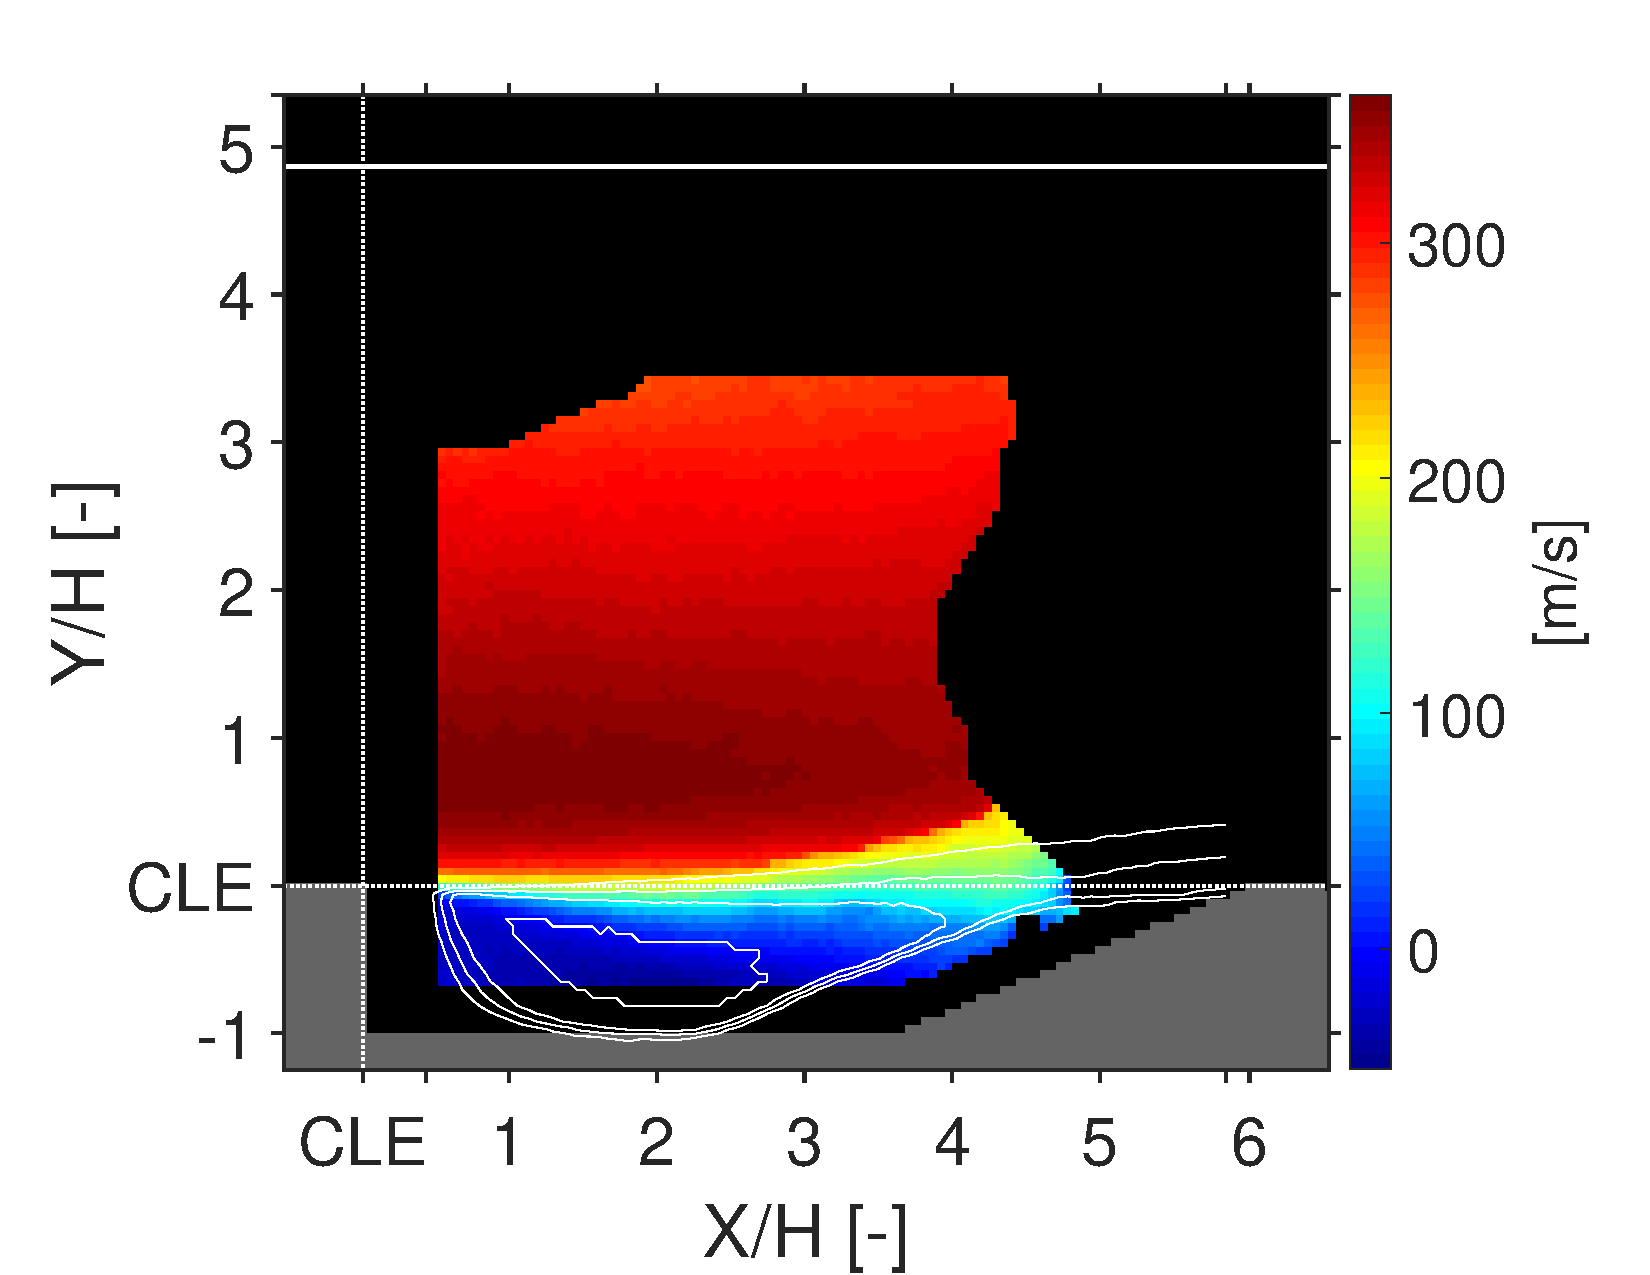
\includegraphics[width=3in,trim=0.35in 0 0.42in 0, clip]{figures/B1/whole_statistics/B1_Ux_AVG}}
         \hspace{0.4in}
\subcaptionbox{Transverse mean velocities.\label{fig:B1_Uy_AVG}}
         {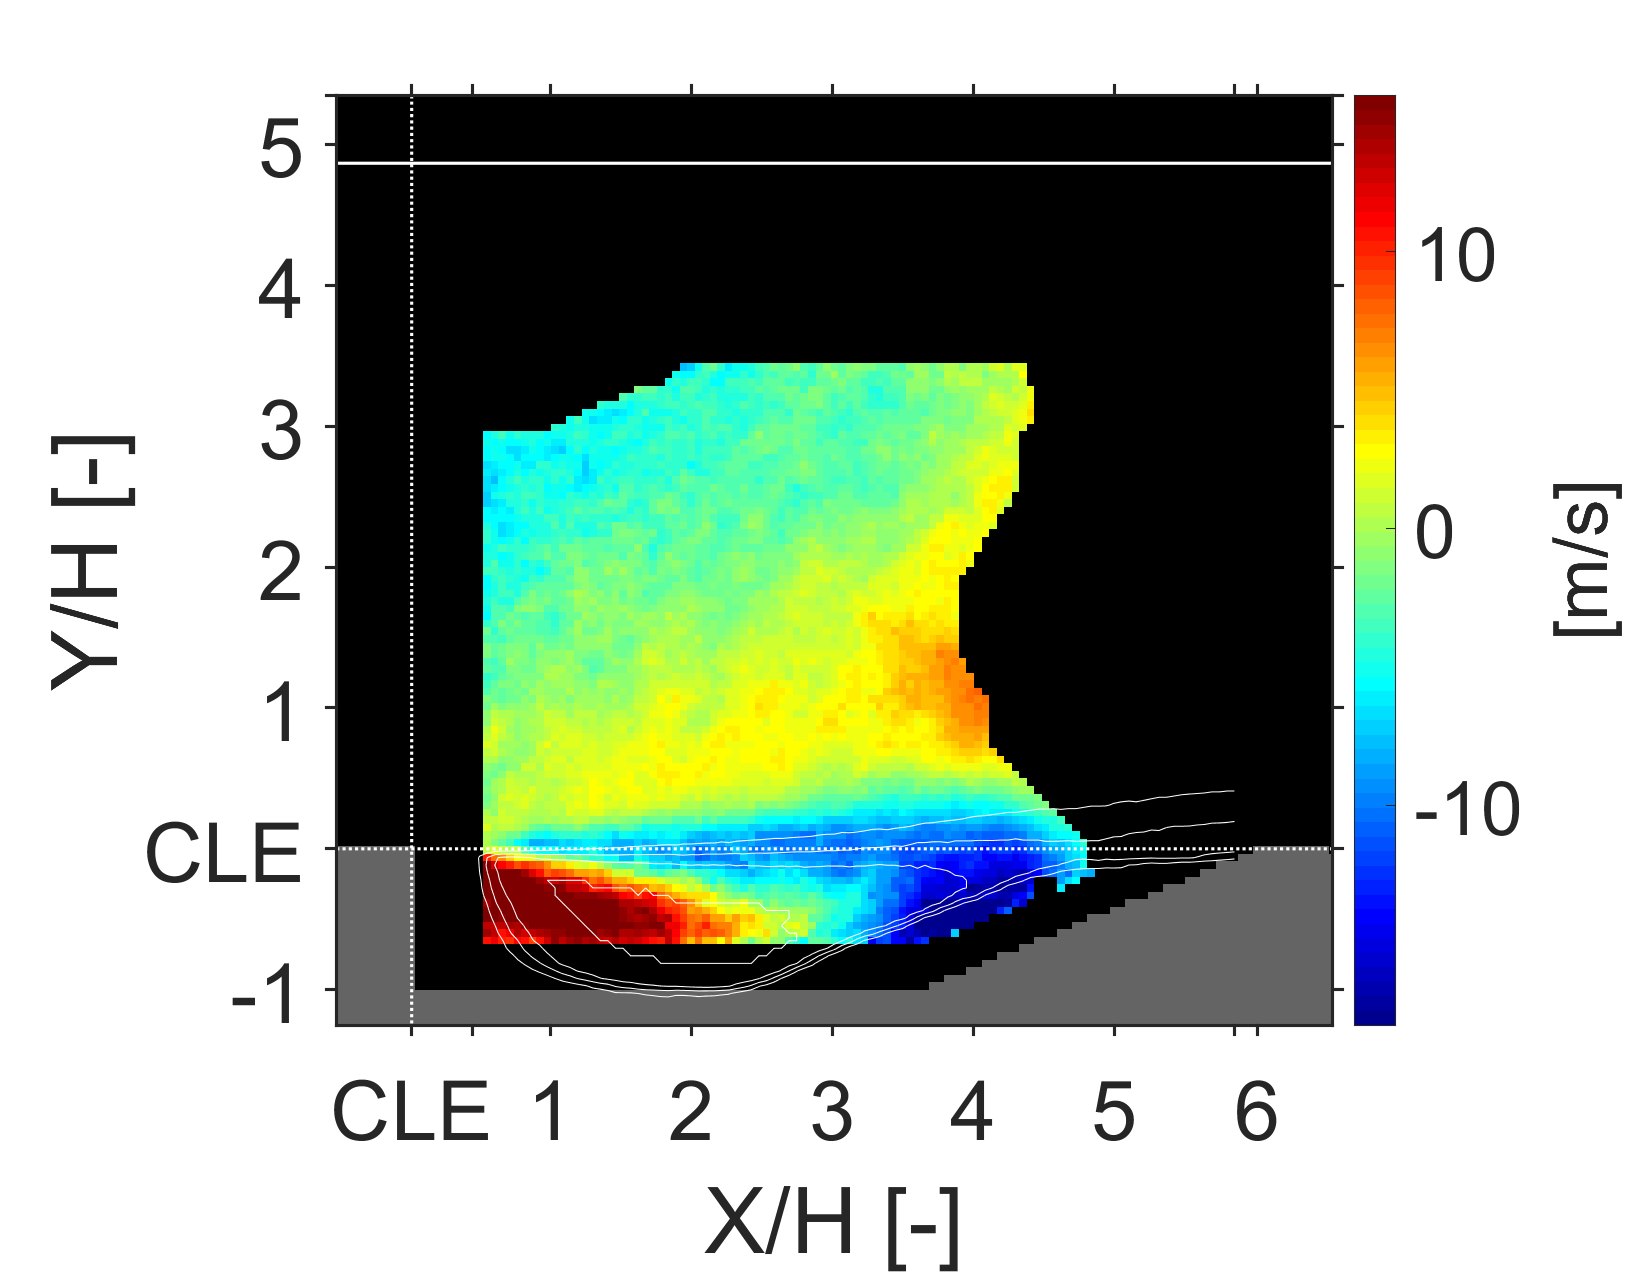
\includegraphics[width=3in,trim=0.35in 0 0.42in 0, clip]{figures/B1/whole_statistics/B1_Uy_AVG}}
         \newline
        \subcaptionbox{Mean OH-PLIF signal overlayed with select PIV vectors and streamlines.\label{fig:B1_PLIF}}
{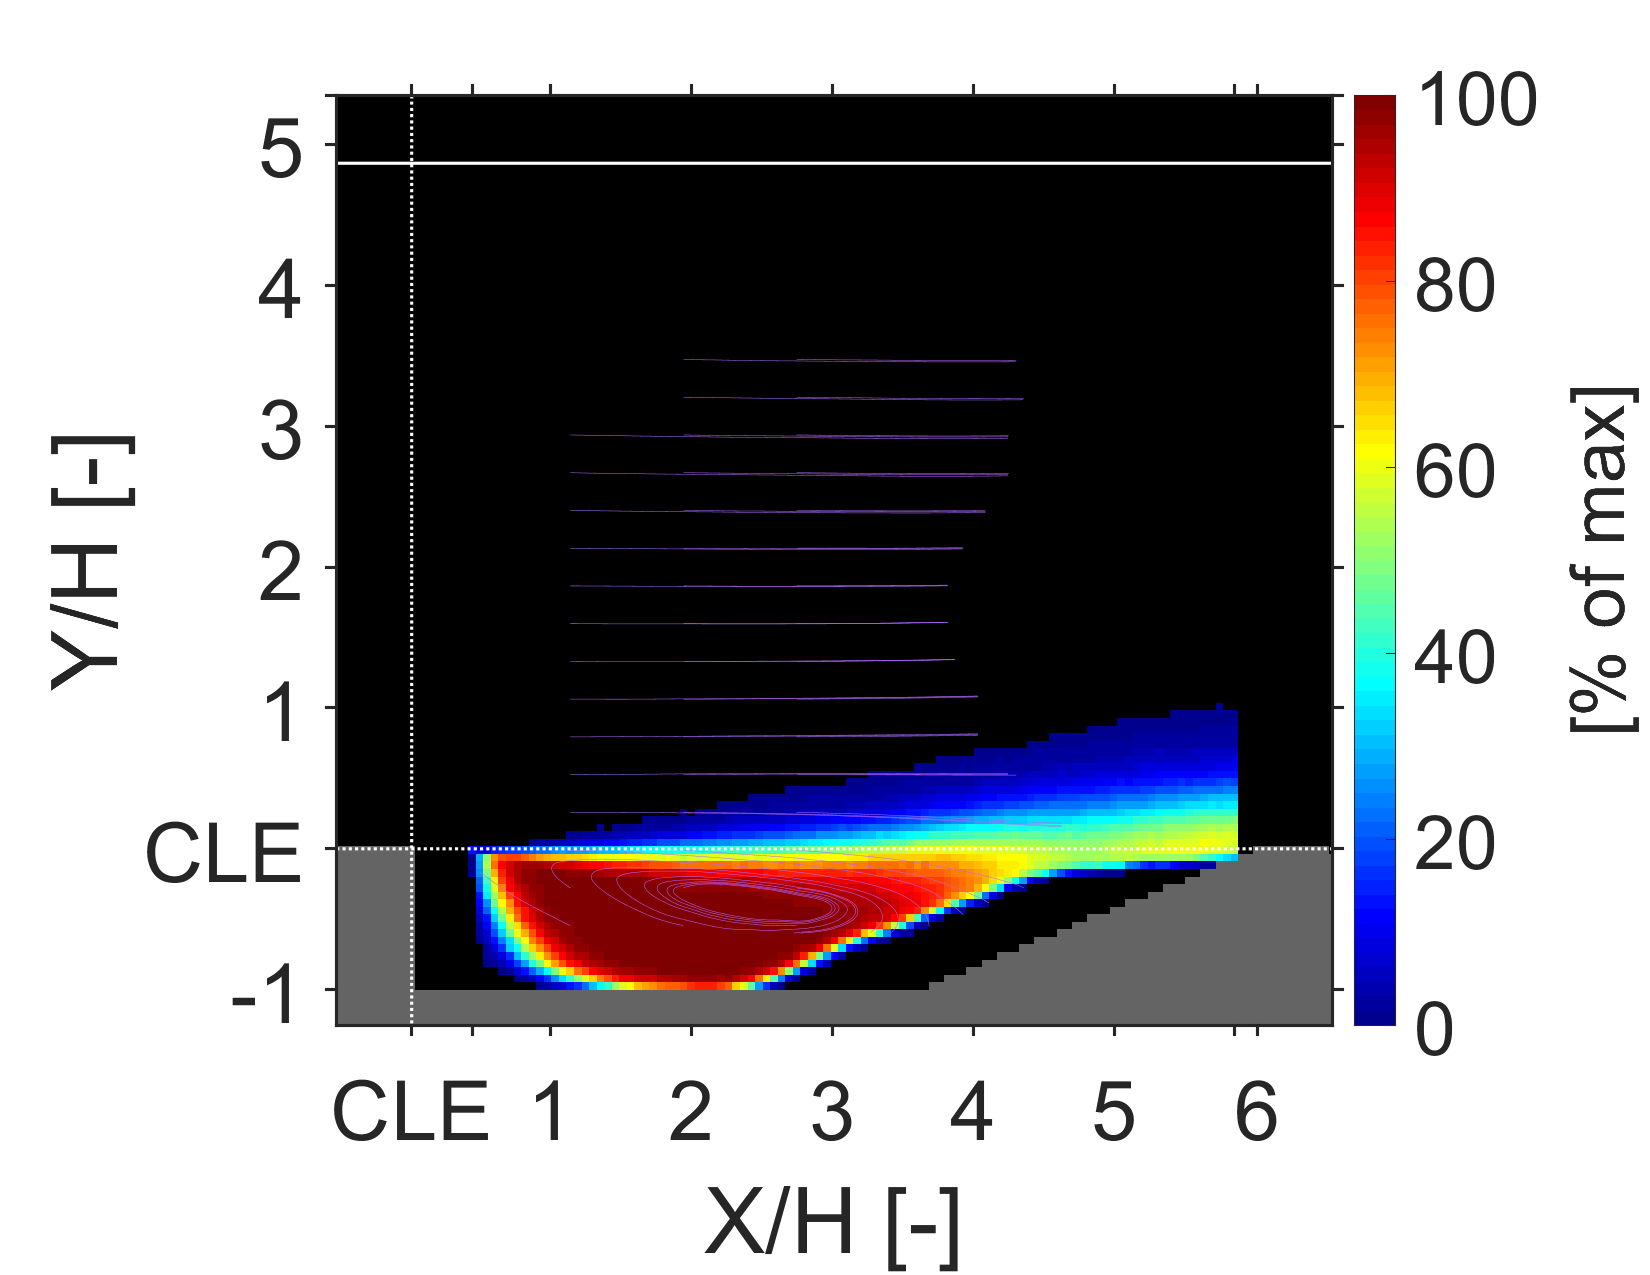
\includegraphics[width=3in,trim=0.35in 0 0.42in 0, clip]{figures/B1/whole_statistics/B1_PLIF}}
         \hspace{0.4in}
\subcaptionbox{Number of good velocity measurements per interrogation window.\label{fig:B1_PLIF2}}
{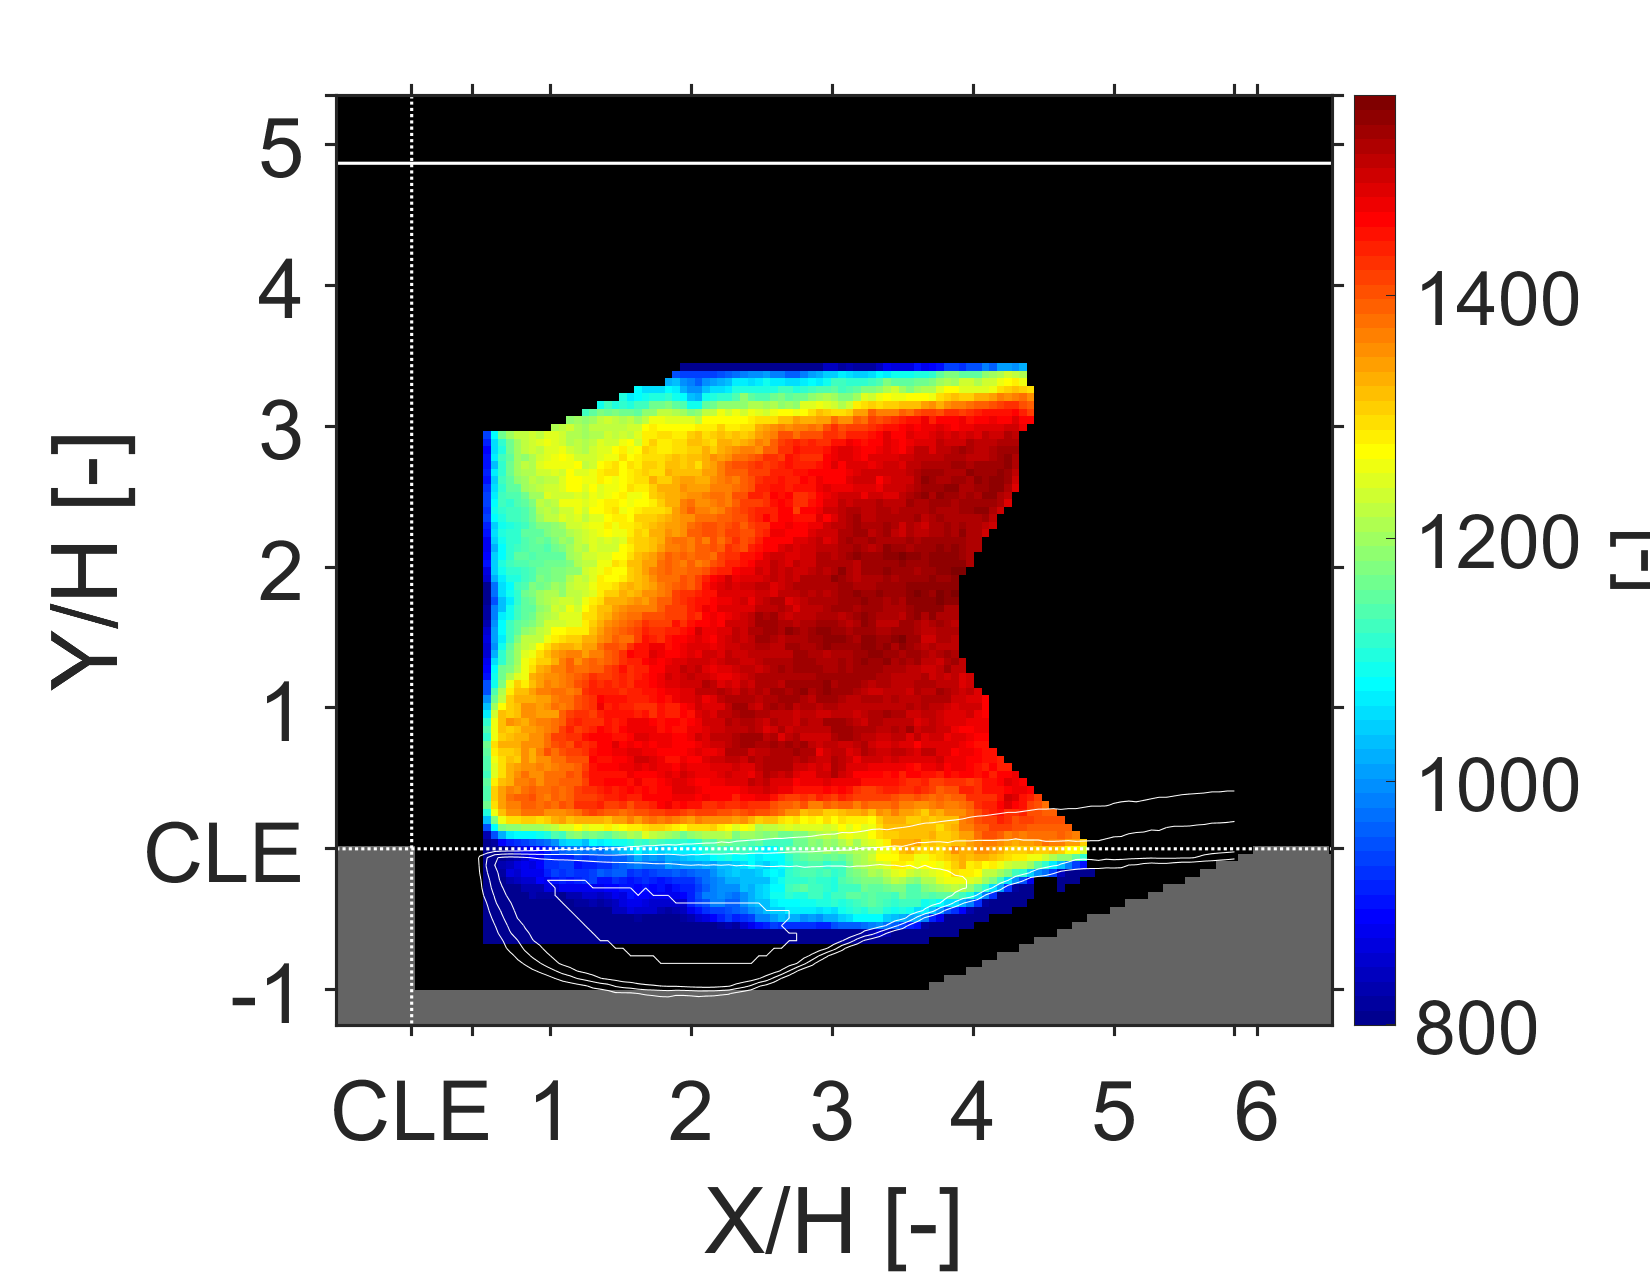
\includegraphics[width=3in,trim=0.35in 0 0.2in 0, clip]{figures/B1/whole_statistics/B1_sample_size}}
\newline
        \subcaptionbox{Fraction of good velocity measurements that are in the products.\label{fig:B1_relative_sample_size}}
{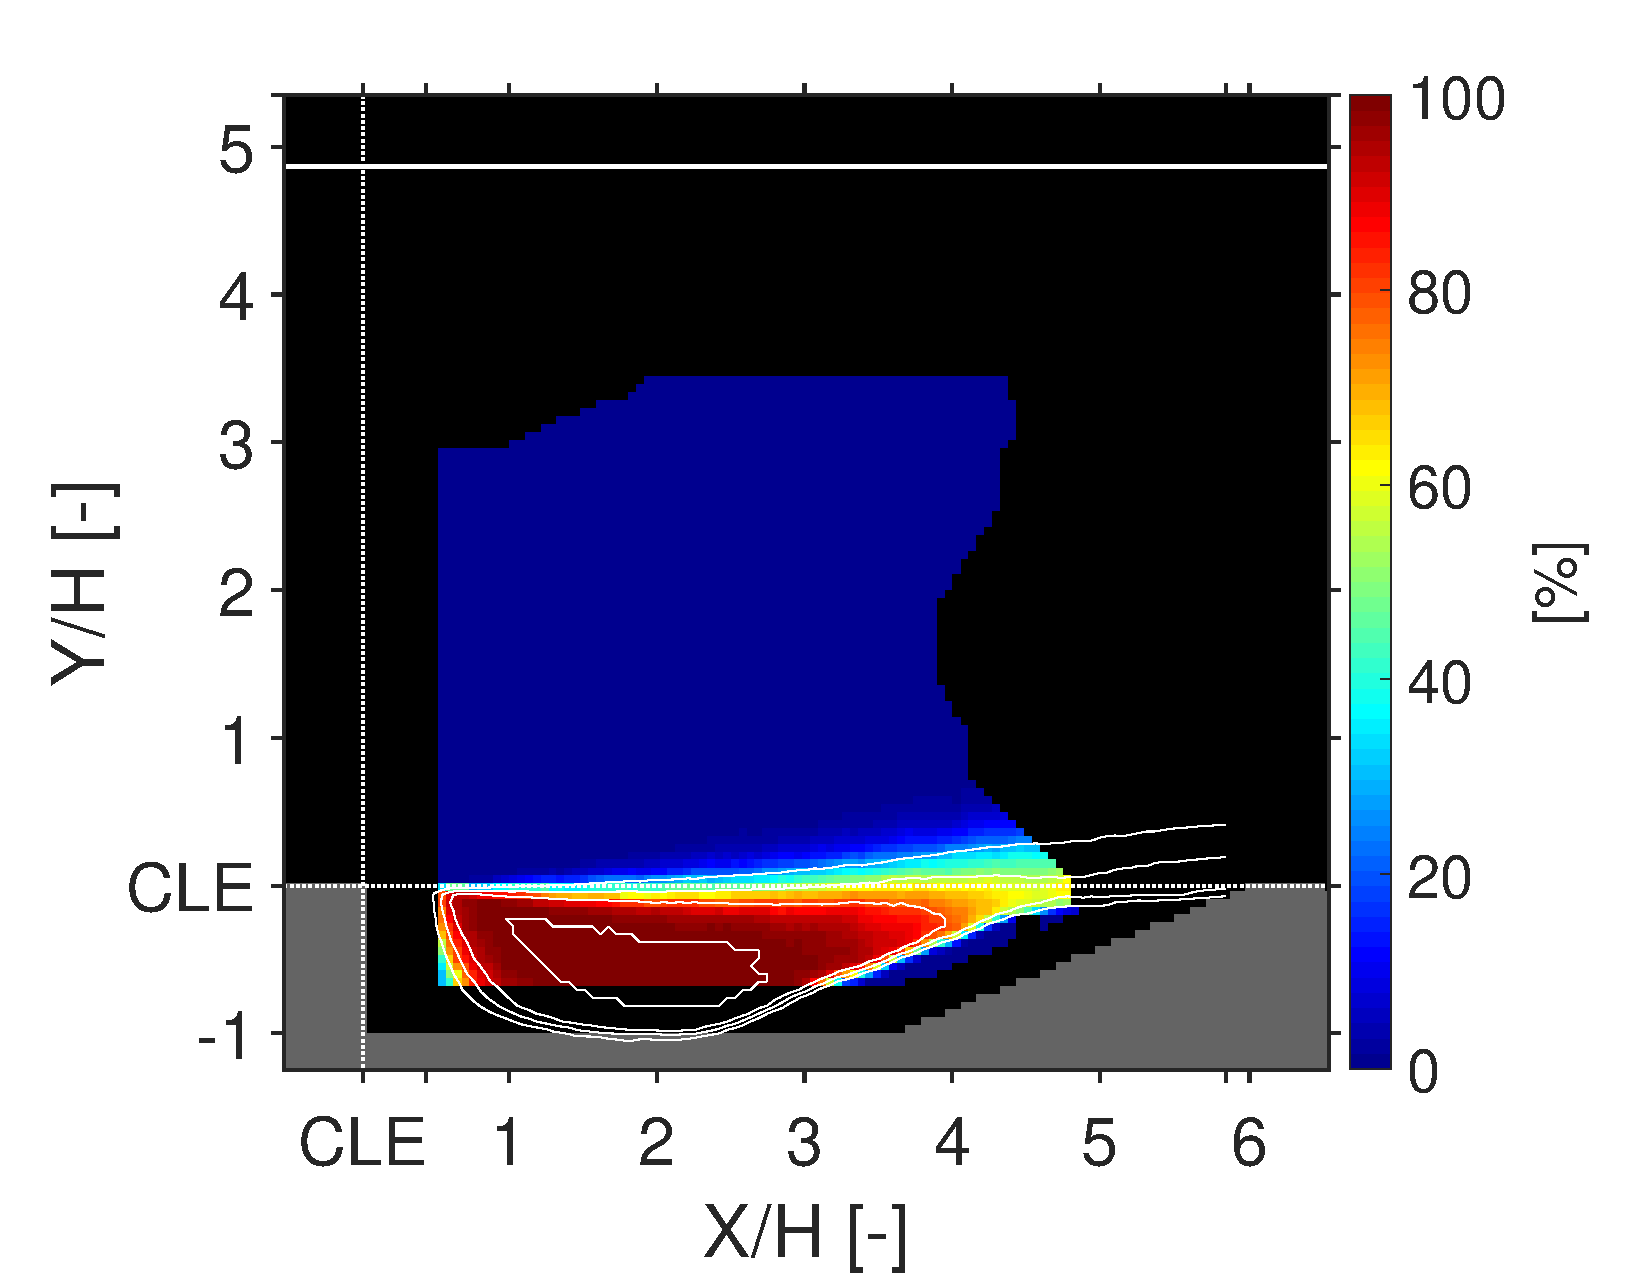
\includegraphics[width=3in,trim=0.35in 0 0.42in 0, clip]{figures/B1/cond_statistics/B1_relative_sample_size}}
\caption{Mean velocity fields with flame intermittency contours}\label{fig:ch3_UxAVG_PIVPLIF}
\end{figure}

\subsection*{Fluctuations}
Figure \ref{fig:ch3_UxRMS_PIVPLIF} displays the field of the velocity RMS, representative of flow fluctuations.  Uncertainties in the axial velocity for a 95$\%$ confidence interval are in the range $\pm5$ to 10$\%$ and for the transverse velocity are in the range $\pm6$ to 10 $\%$.  RMS values in the flow above the shear layer are similar to the inflow values measured at $x/H=-1.6$ presented in \cite{LieberThesis}. The axial and transverse fluctuations in the main duct flow increase towards the opposite wall due to the presence of the thick boundary layer. The main duct flow also shows turbulent anisotropy with $U_{y,~ RMS}$ in the range 30 to 35 m/s and $U_{x,~ RMS}$ in the range 50 to 55 m/s at $y/H=2.5$. 
The axial RMS velocity is highest in the shear layer and lowest in the upstream cavity corner. Peak values are found past $x/H=3$ above the cavity regions, hinting at disrupting product ejection events as observed in instantaneous PLIF measurements. 
A large region of heightened transverse RMS velocities coincides with the upper half of the elliptical recirculation region. Peak transverse RMS velocities occur on the ramp indicating shear layer impingement, in agreement with previous observations \citep{Kirik2017}. Similarly to the axial RMS, the transverse RMS drops in the cavity upstream corner where a small low-speed recirculation region was identified in a larger cavity \citep{Kirik2017}. Based on observations from \citet{Kirik2017}, this portion of the cavity is expected to be filled by hot, burned gases that are forced toward the front of the cavity by the recirculation process. These gases provide an ignition source for the fresh fuel-air mixture as they are entrained by the main recirculation zone into the cavity shear layer.

\begin{figure}
\centering
\subcaptionbox{Axial RMS velocities.\label{fig:B1_Ux_RMS}}
         {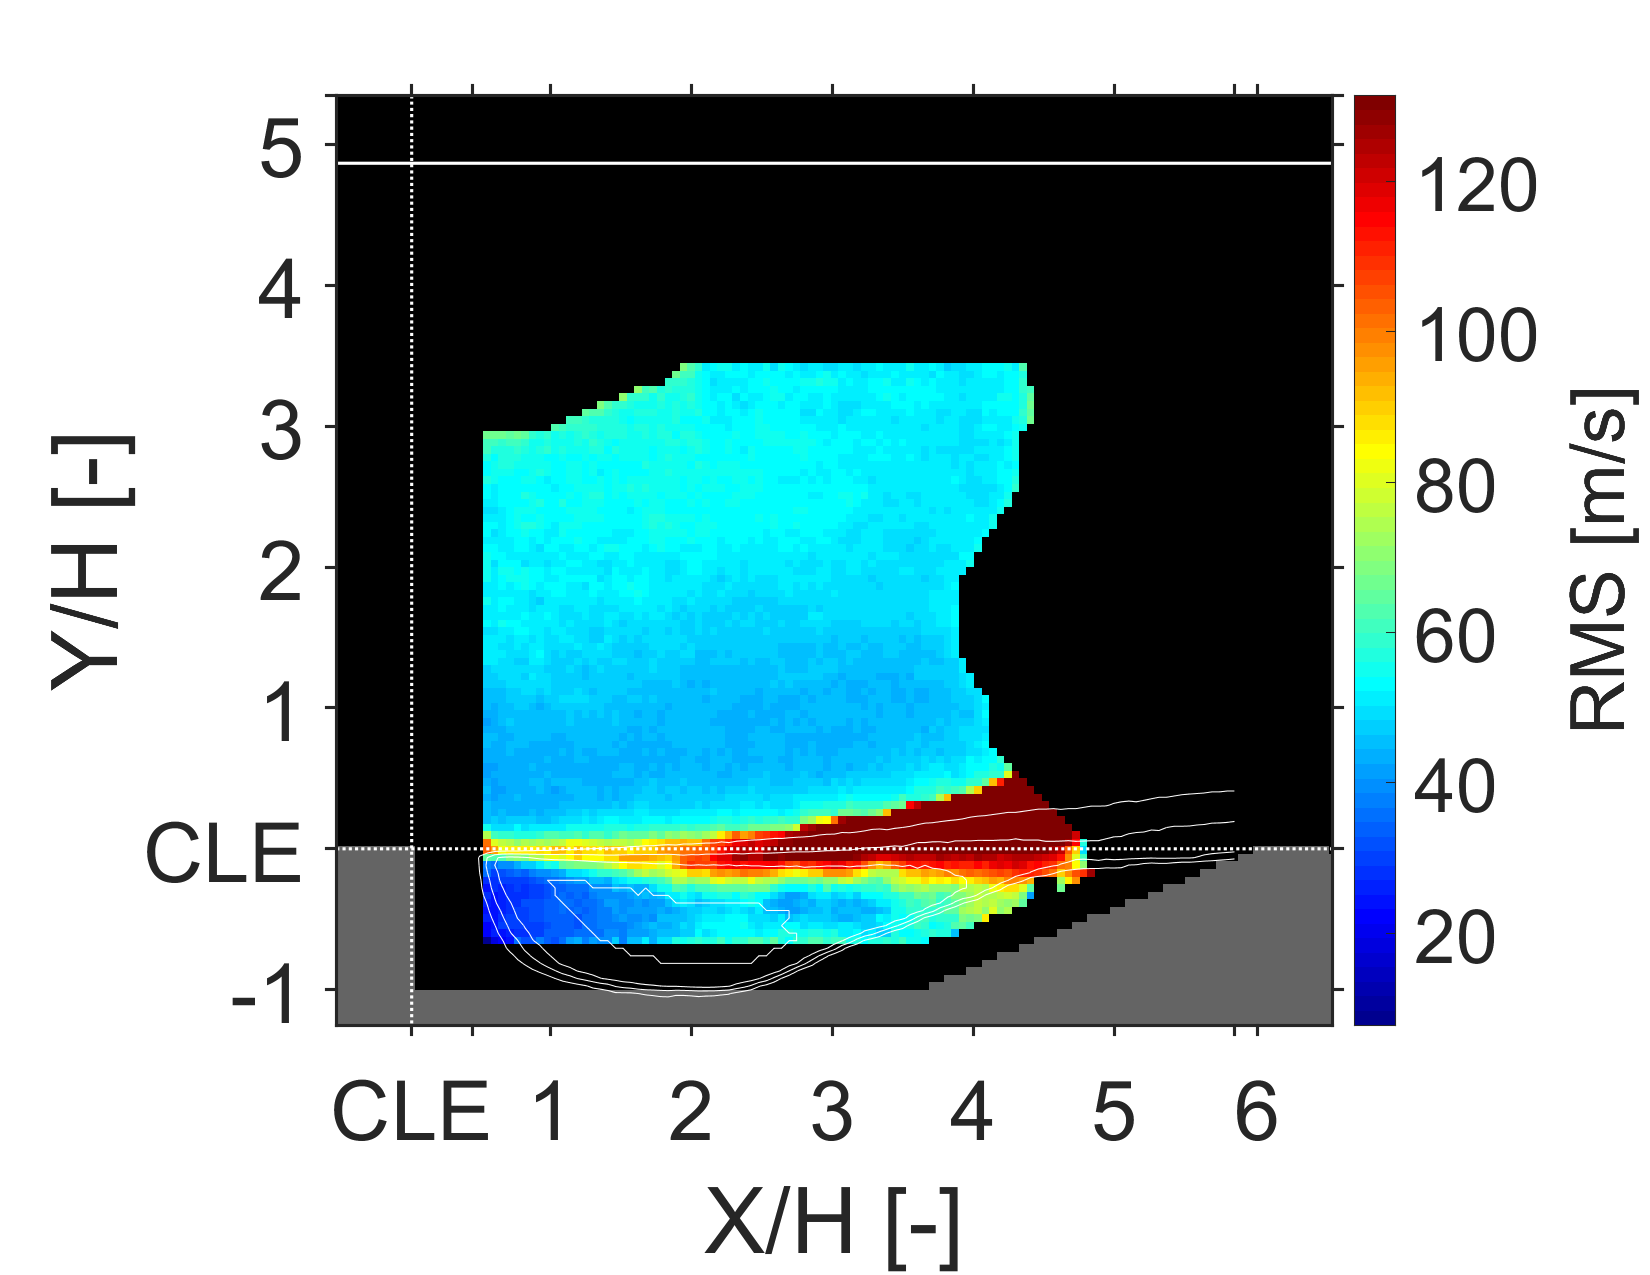
\includegraphics[width=3in,trim=0.35in 0 0.42in 0, clip]{figures/B1/whole_statistics/B1_Ux_RMS}}
        \hspace{0.4in}
\subcaptionbox{Transverse RMS velocities.\label{fig:B1_Uy_RMS}}
                {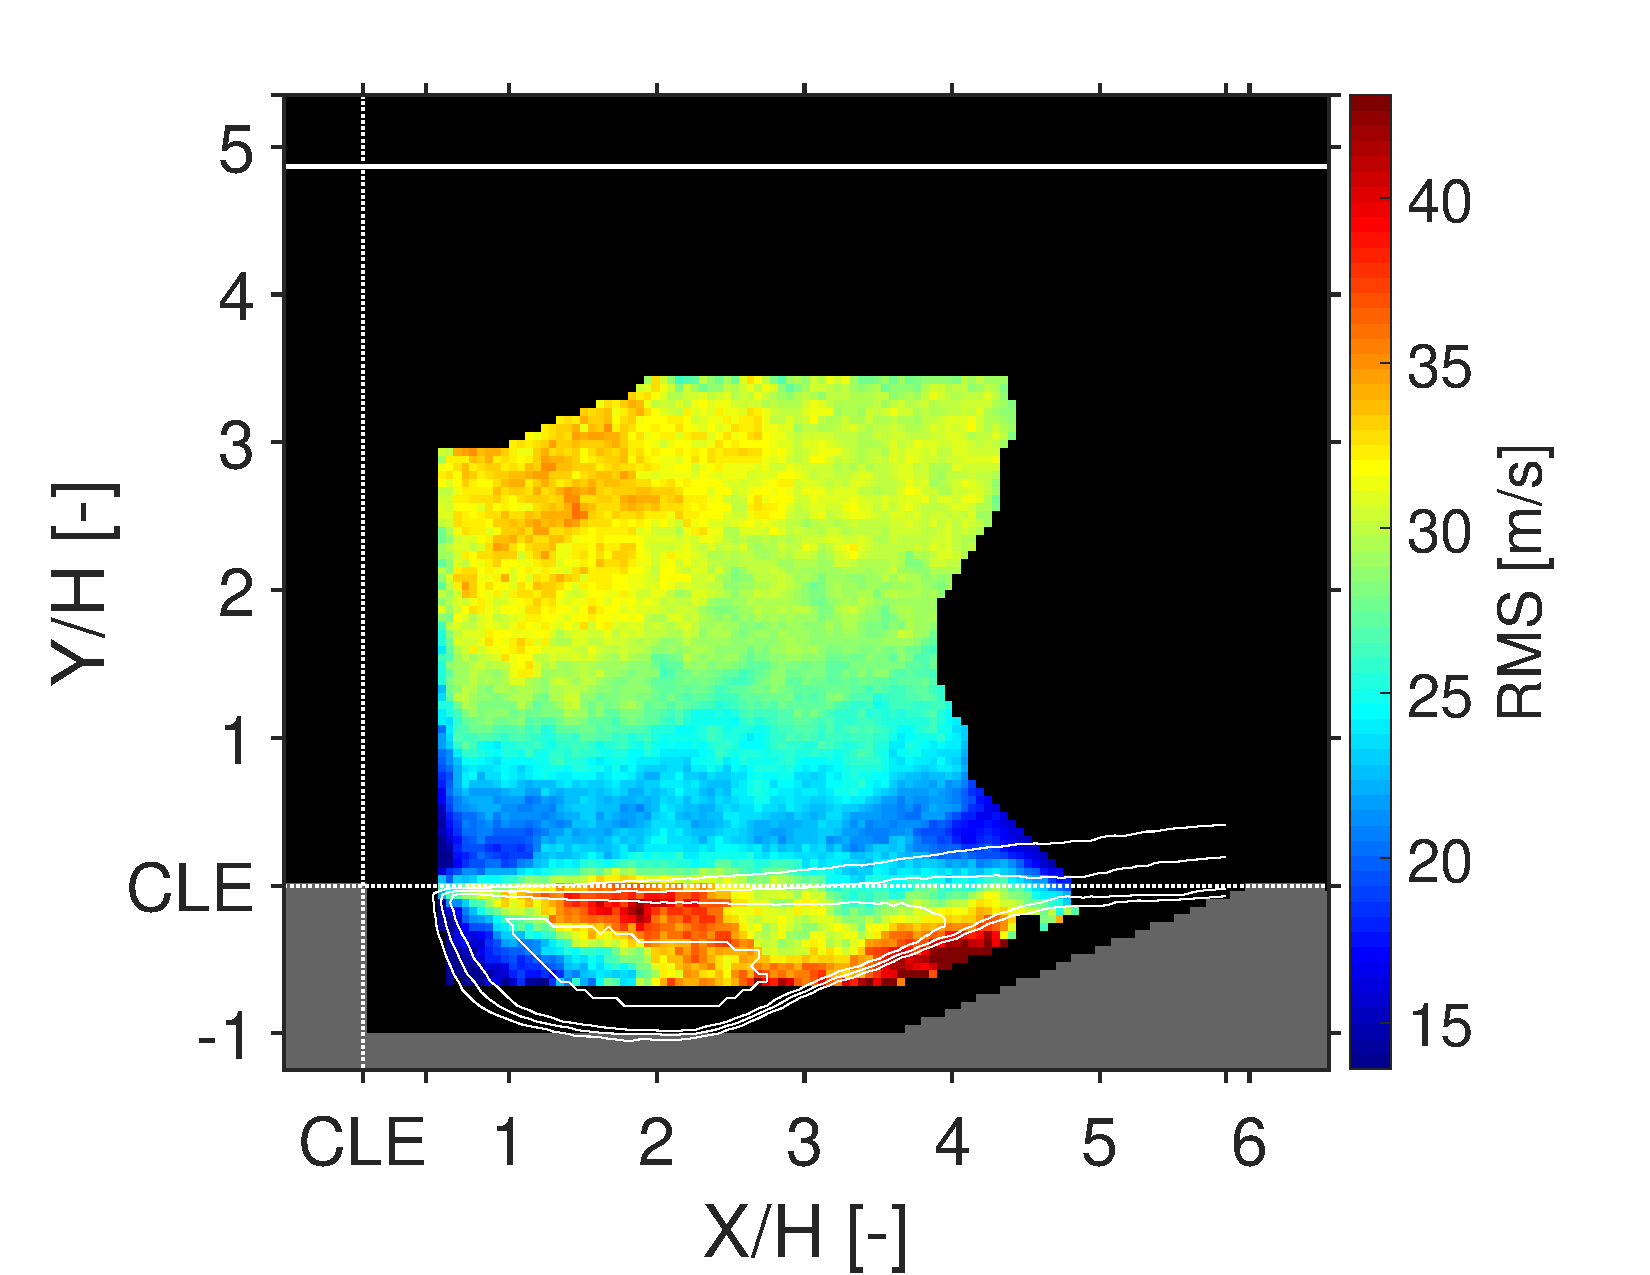
\includegraphics[width=3in,trim=0.35in 0 0.42in 0, clip]{figures/B1/whole_statistics/B1_Uy_RMS}}
\caption{RMS velocity components with flame intermittency contours}\label{fig:ch3_UxRMS_PIVPLIF}
\end{figure}

The turbulence intensity (Fig. \ref{fig:B1_Ux_TI}) displays a strong increase along the elliptical recirculation region major axis. Values exceeding 200$\%$ are detected in those areas, versus the main duct flow values of 10-15$\%$.  In contrast, the turbulent kinetic energy follows the trends of the axial fluctuations, i.e. with high values in the shear layer and a peak in the regions of product ejection. Uncertainties in the turbulence intensity are $\sim 4\%$ in duct flow and $<10\%$ in cavity (except on the elliptical recirculation zone axis).

\begin{figure}
\centering
\subcaptionbox{Turbulence intensities.\label{fig:B1_Ux_TI}}
        {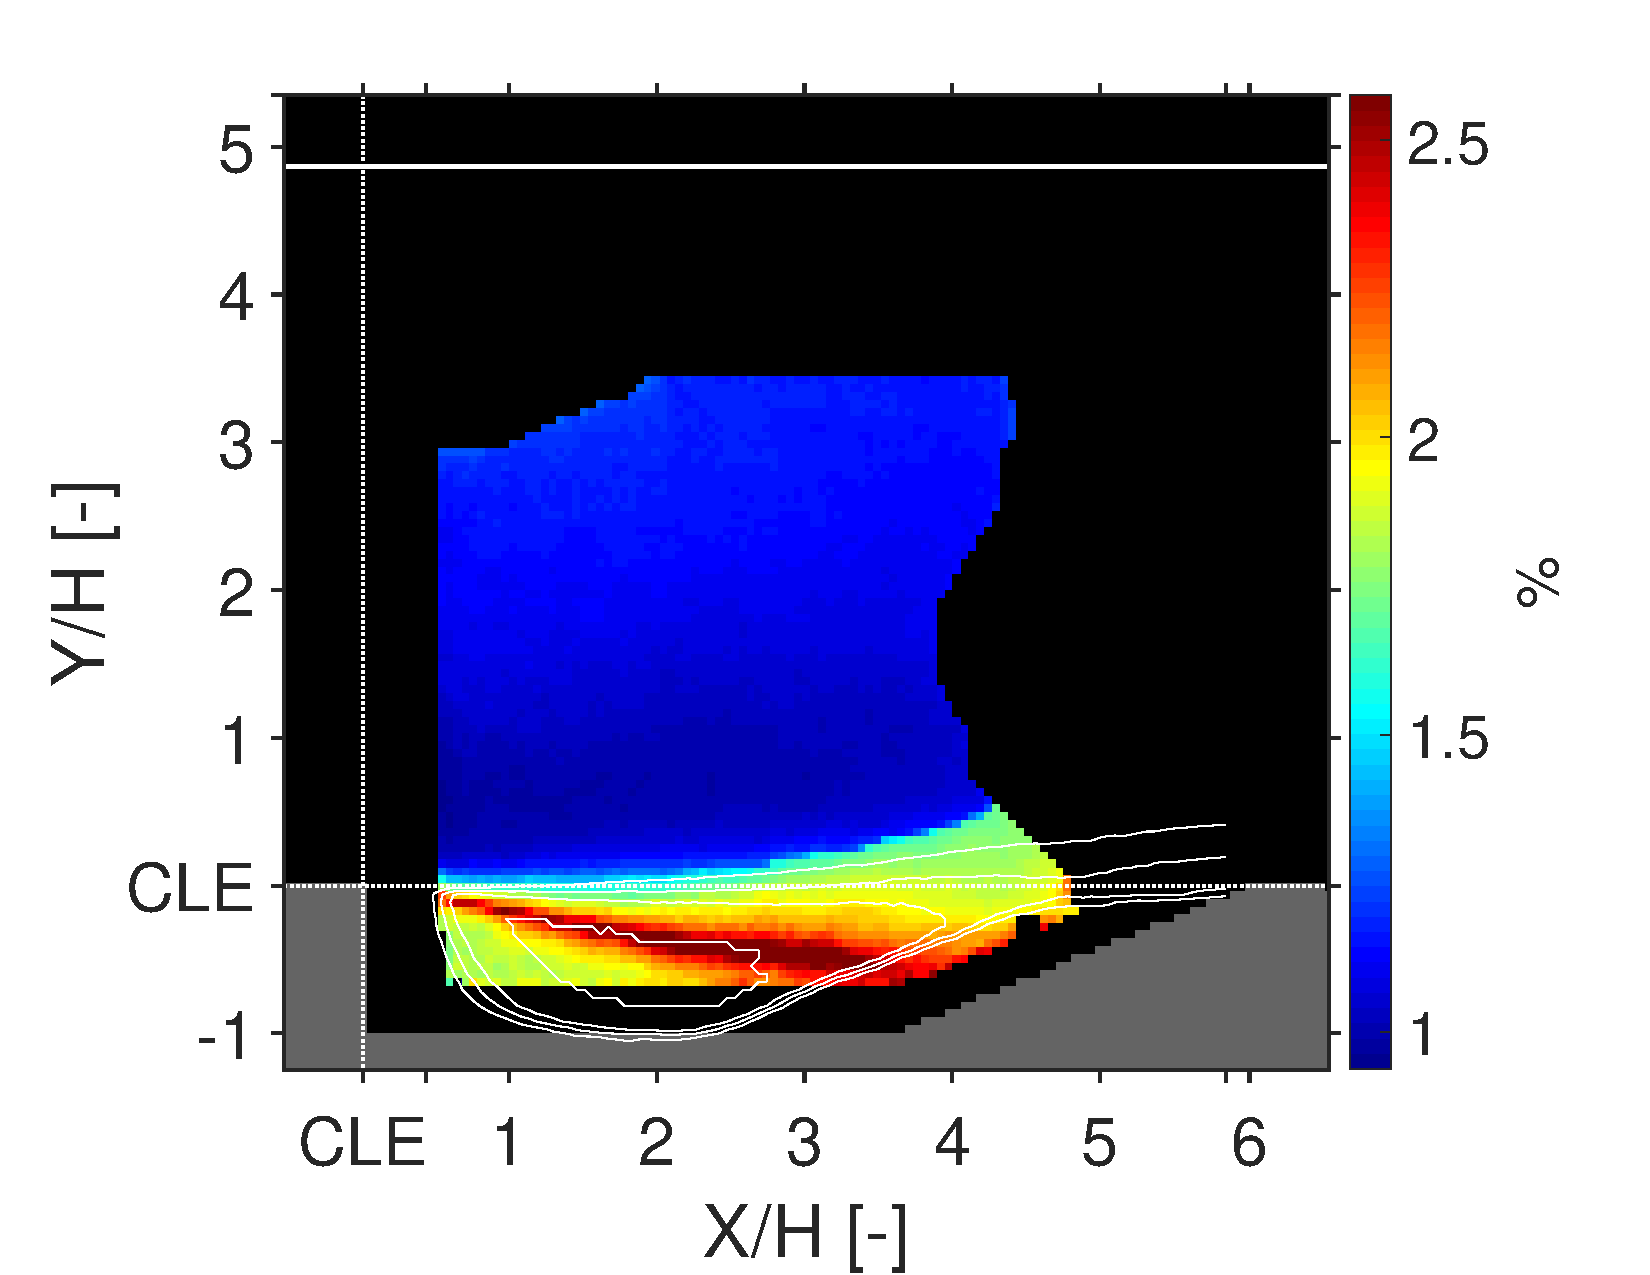
\includegraphics[width=3in, trim=0.3in 0in 0.1in 0.1in, clip]{figures/B1/whole_statistics/B1_TI}}
        \hspace{0.2in}
\subcaptionbox{Turbulent kinetic energy.\label{fig:B1_Uy_TKE}}
{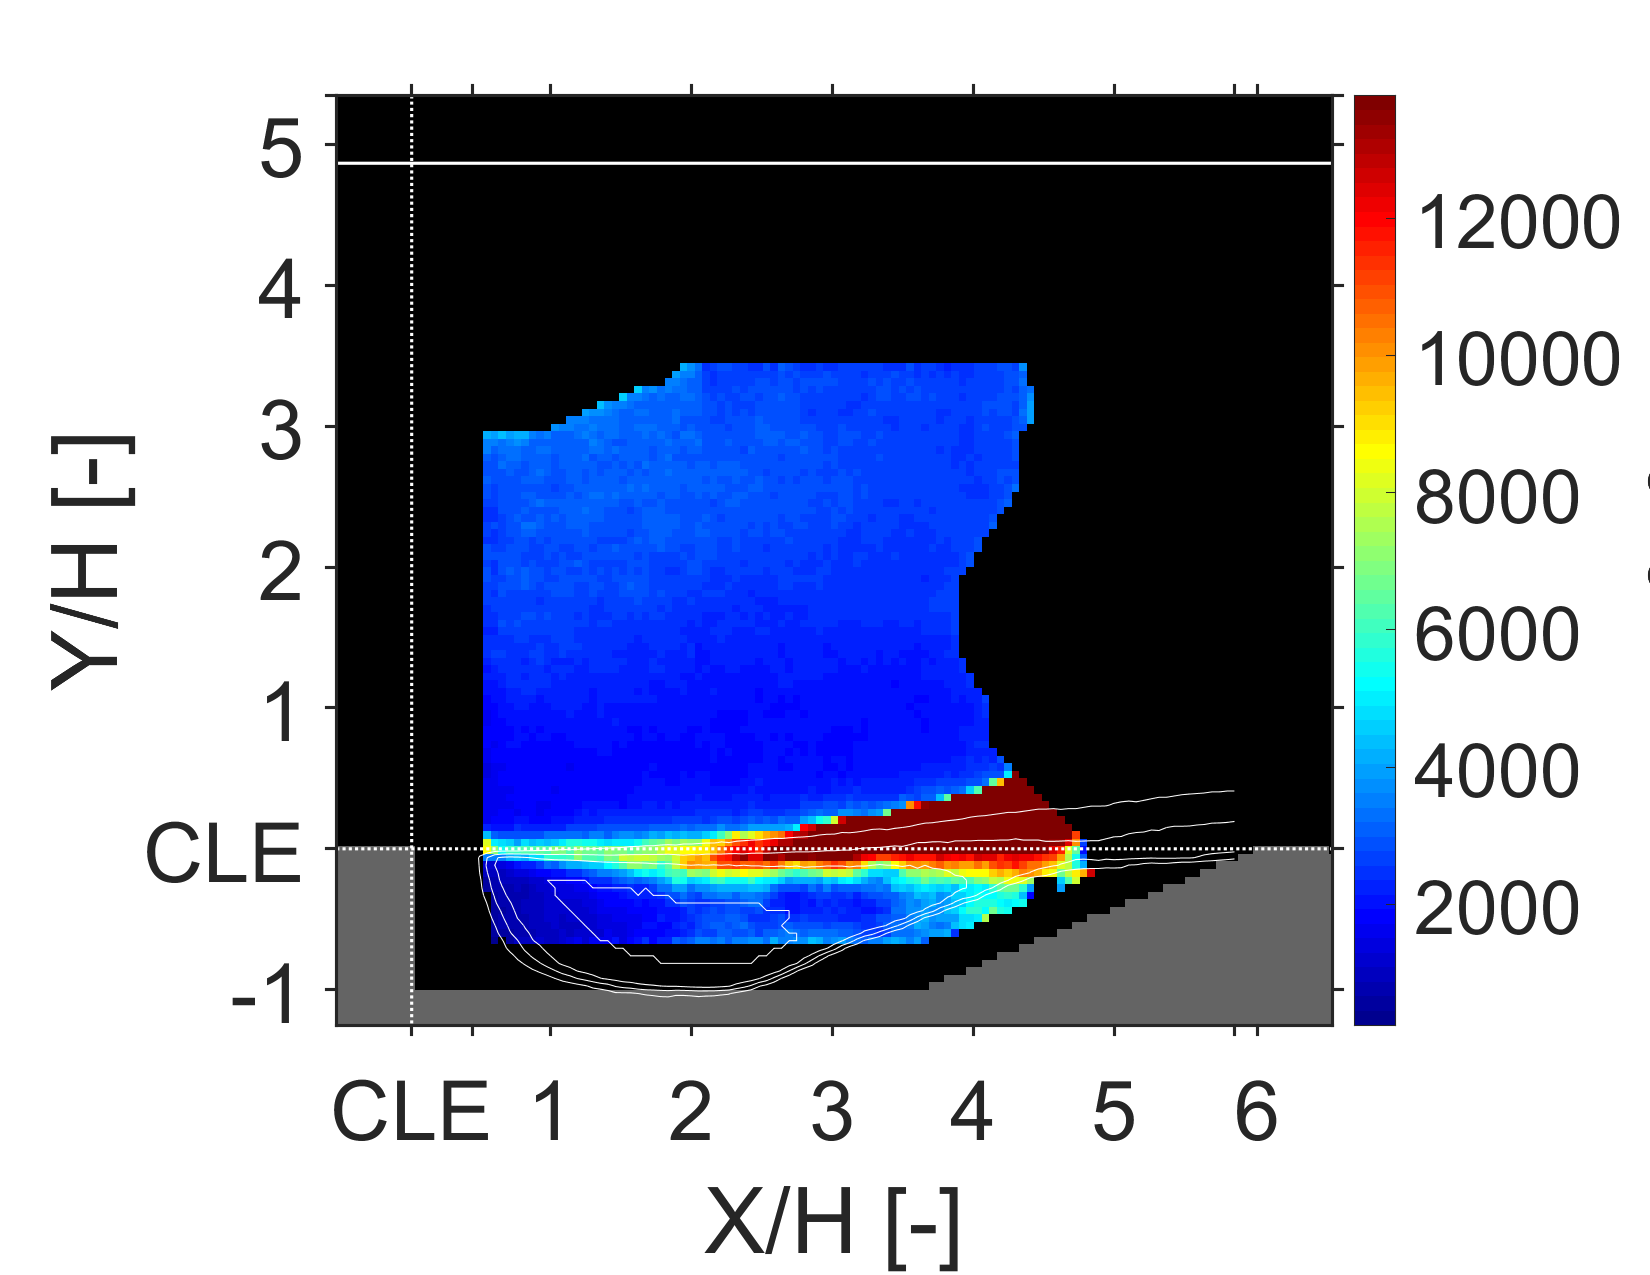
\includegraphics[width=3in,trim=0 0 1.3cm 0, clip]{figures/B1/whole_statistics/B1_TKE}
\rotatebox{90}{\hspace{1.15in}\footnotesize$\mathrm{[m^2/s^2]}$}}
\caption{Fluctuation energy indicators with flame intermittency contours}\label{fig:ch3_UxTKETI_PIVPLIF}
\end{figure}

\subsection*{Conditional velocities}\label{sec:ch3_cond_vel}
Figure \ref{fig:B2_all_cond_AVG} shows the mean absolute and relative conditional velocities with overlayed flame intermittency contours in white. The reactants and products axial velocity values and trends are similar to each other (see Figs. \ref{fig:B1_Ux_AVG_reactants} and \ref{fig:B1_Ux_AVG_products}), while the reactant transverse velocities below the cavity-freestream interface indicate reactants are entering the cavity and the product transverse velocities above the cavity-freestream interface indicate that products are escaping the cavity (see Figs. \ref{fig:B1_Uy_AVG_reactants} and \ref{fig:B1_Ux_AVG_products}). Transverse velocities are negative for both the products and reactants in the shear layer (Figs. \ref{fig:B1_Uy_AVG_reactants} and \ref{fig:B1_Uy_AVG_products}), but these velocities may change sign towards the aft end of the ramp where measurements were not possible. The difference between the reactant and the product mean velocities (Figs. \ref{fig:B1_relative_Ux_AVG_conditional} and \ref{fig:B1_relative_Uy_AVG_conditional}) indicates an upwards and backwards flow of the products relative to the reactants with mean velocity on the order of 1-10 m/s, in which reactants flow into products regions to ignite, transform into products, and flow out against incoming premixed flow.

Analysis of mass flux can reveal whether mass is accumulated and subsequently ejected at the cavity-freestream boundary. Because the measurement is two-dimensional, no spanwise flow can be taken into account.  The mass flux calculation also requires knowledge of the density, unavailable from the present measurements. Nonetheless, the direction of mass transfer may be inferred from the average transverse velocity at the cavity interface at $y/H=0$, shown in Fig. \ref{fig:ch3_cavity_interface_flux}. 
Both the products and reactants are on average flowing into the cavity with the exception of the region closest to the CLE, where velocities are zero. The hidden region past $x/H=5$ is expected to follow the increasing trend seen between $x/H=$ 4 to 5 in Fig. \ref{fig:ch3_cavity_interface_flux} such that the mean transverse flux along the entire cavity interface equals zero and mass is conserved. Therefore, mass transfer out of the cavity mostly occurs near the ramp. This observation, in conjunction with the 60$\%$ flame intermittency at the downstream end of the cavity interface (see Fig. \ref{fig:B1_PLIF}), hints at ejection events that compensate for the mass and heat accumulated in the cavity over the remaining 40$\%$ of the time. Ensemble statistics do not allow further investigation into the disrupting ejection events suggested by the above results. In the following section, the problem is further studied using instantaneous measurements.

\begin{figure}
\centering
        \subcaptionbox{Reactants $\bar{U}_{x,R}$\label{fig:B1_Ux_AVG_reactants}}
        {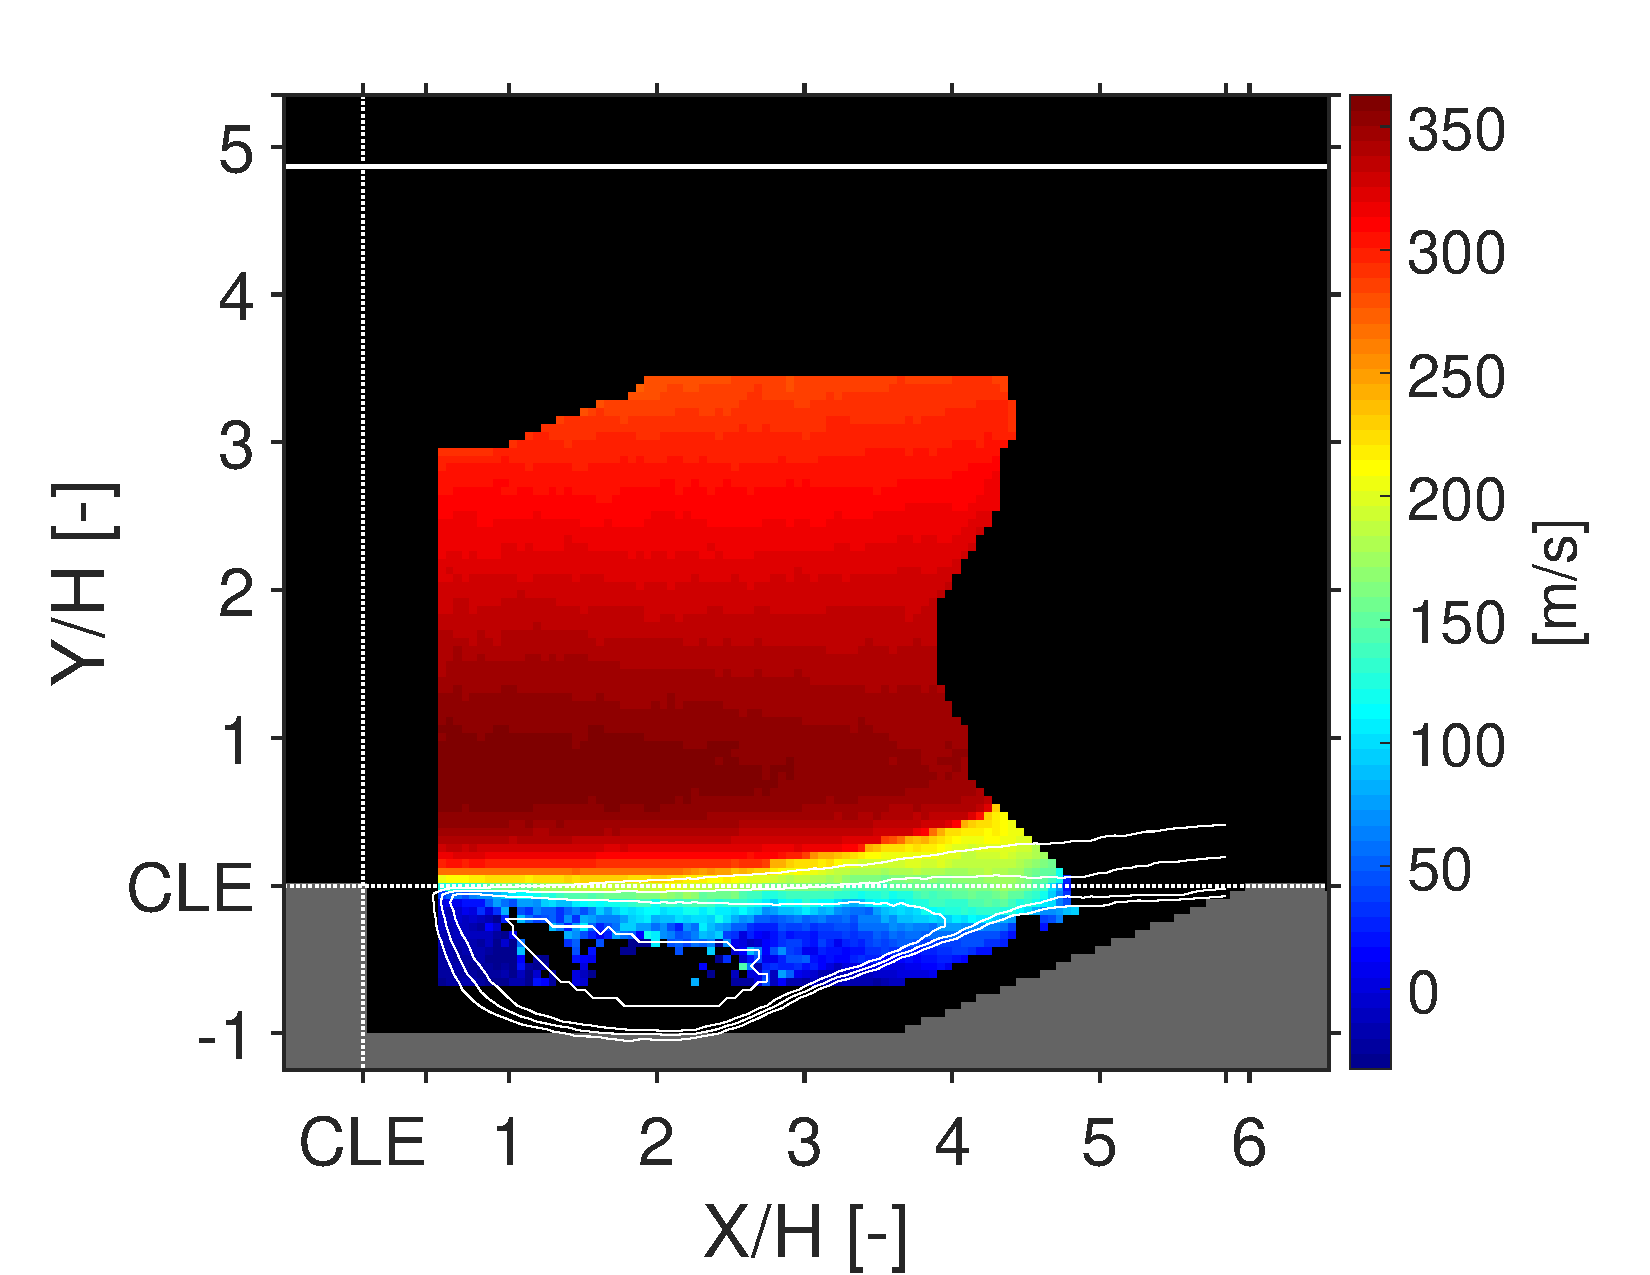
\includegraphics[width=3in,trim=0.35in 0 0.42in 0, clip]{figures/B1/cond_statistics/B1_Ux_AVG_reactants}} \hspace{0.4cm}
        \subcaptionbox{Products $\bar{U}_{x,P}$\label{fig:B1_Ux_AVG_products}}
        {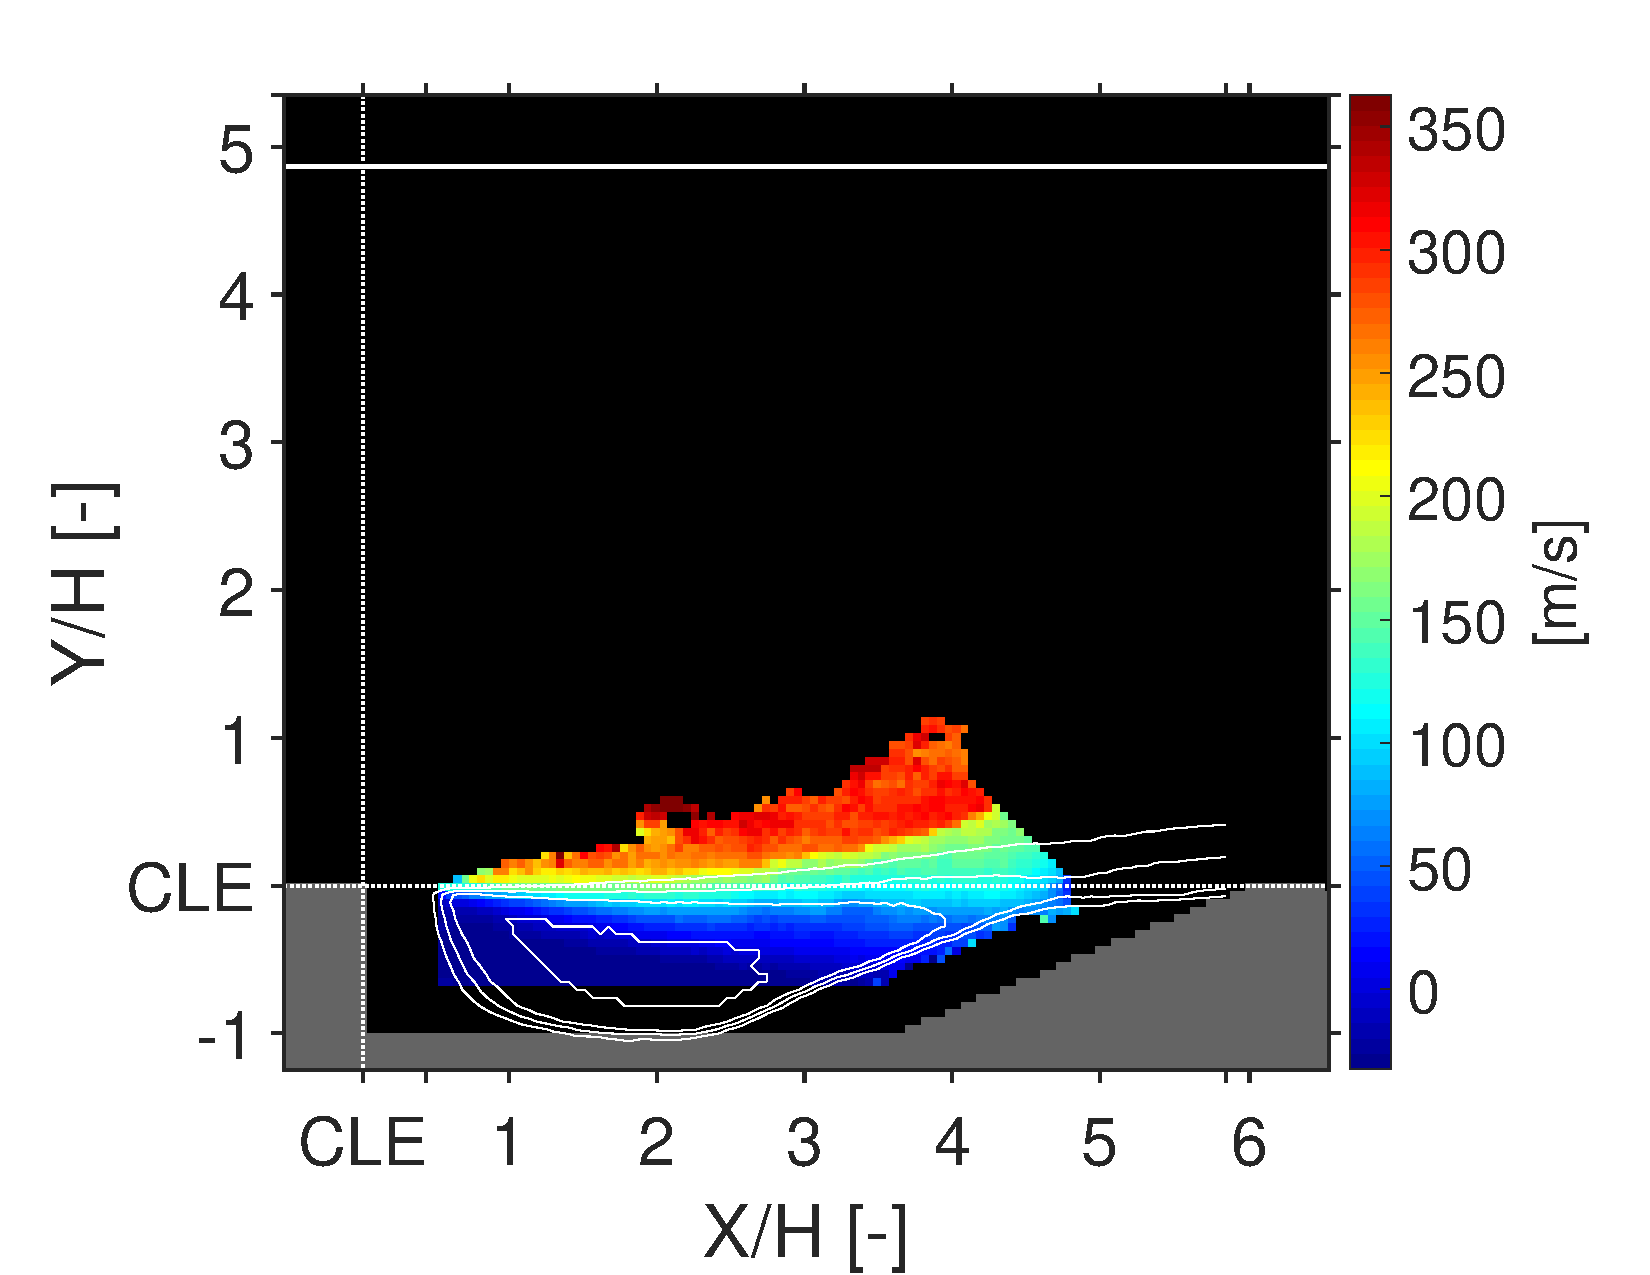
\includegraphics[width=3in,trim=0.35in 0 0.42in 0, clip]{figures/B1/cond_statistics/B1_Ux_AVG_products}}
        \newline
        
        \subcaptionbox{Reactants $\bar{U}_{y,R}$\label{fig:B1_Uy_AVG_reactants}}
        {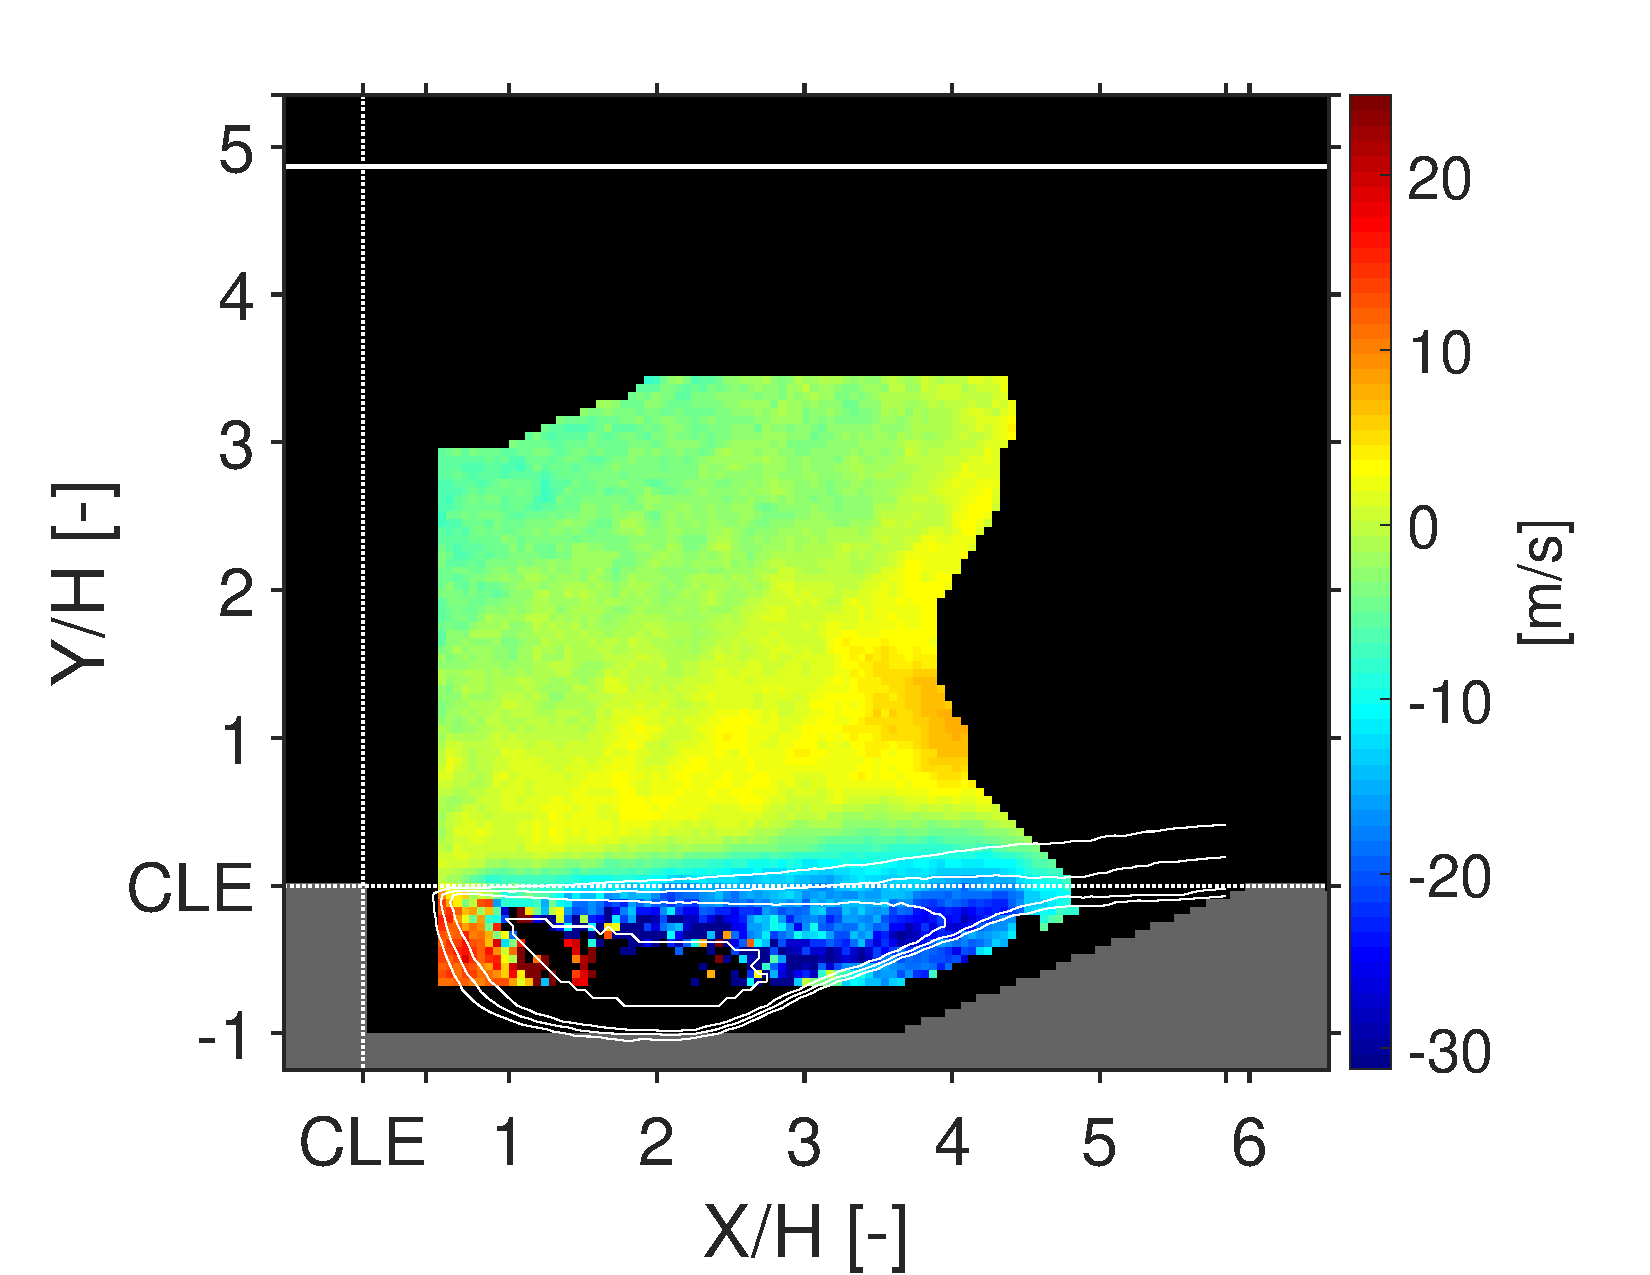
\includegraphics[width=3in,trim=0.35in 0 0.42in 0, clip]{figures/B1/cond_statistics/B1_Uy_AVG_reactants}} \hspace{0.4cm}
        \subcaptionbox{Products $\bar{U}_{y,P}$\label{fig:B1_Uy_AVG_products}}
        {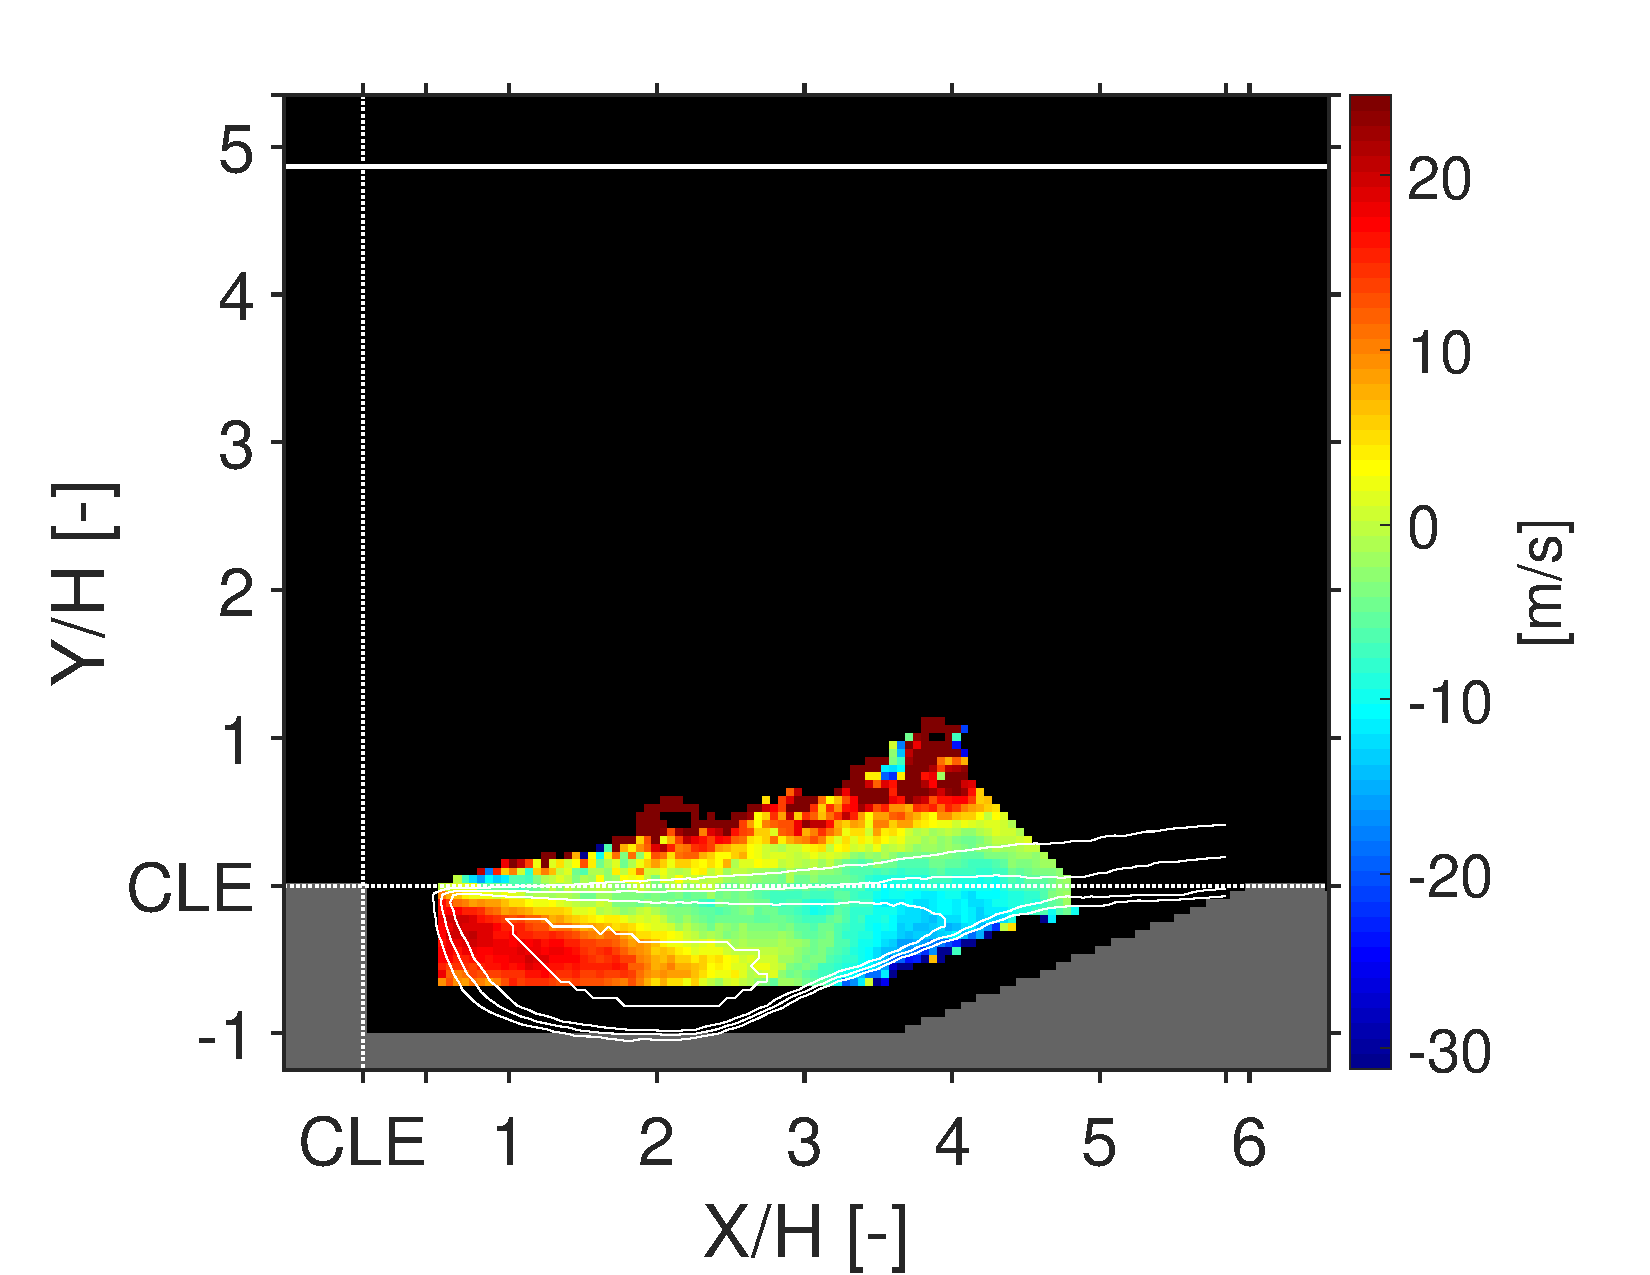
\includegraphics[width=3in,trim=0.35in 0 0.42in 0, clip]{figures/B1/cond_statistics/B1_Uy_AVG_products}}
        \newline
        
        \subcaptionbox{Axial velocities of products relative to reactants \\$\bar{U}_{x,P}-\bar{U}_{x, R}$\label{fig:B1_relative_Ux_AVG_conditional}}
        {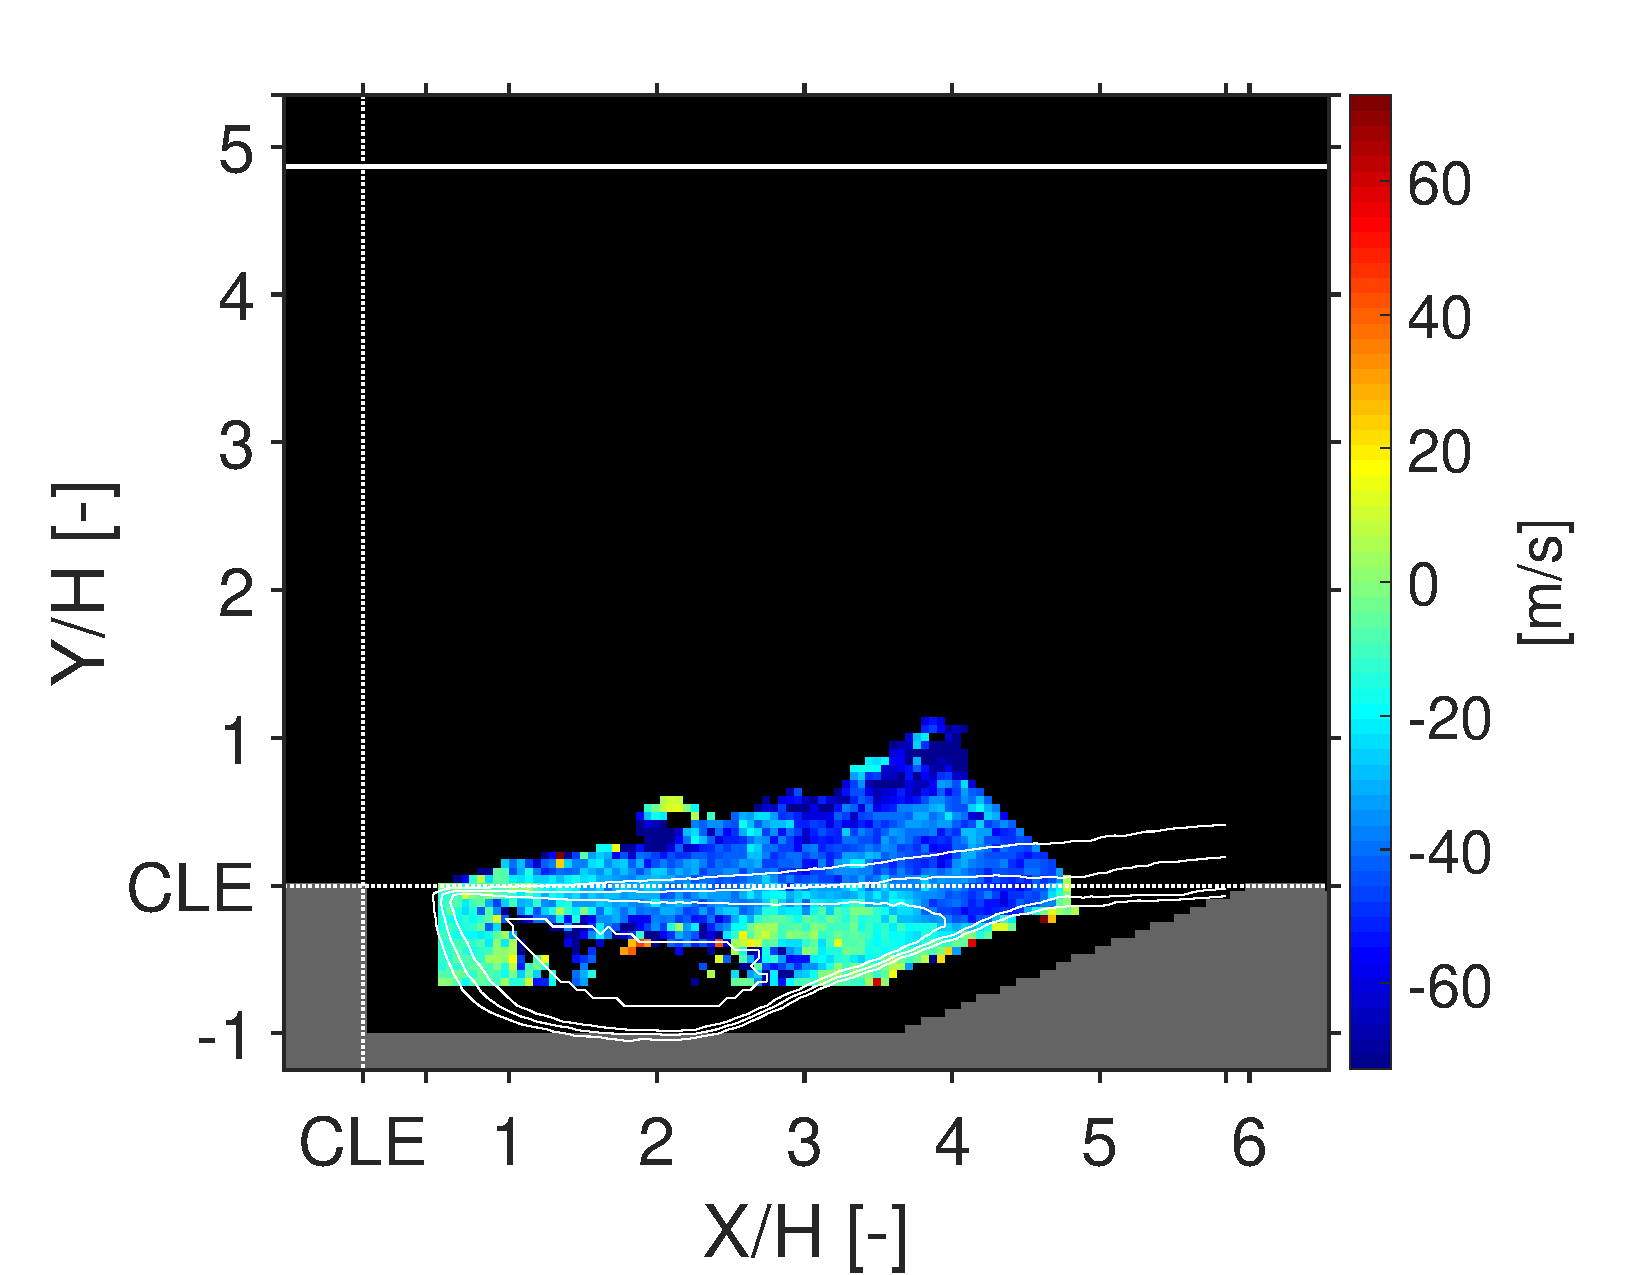
\includegraphics[width=3in,trim=0.35in 0 0.42in 0, clip]{figures/B1/cond_statistics/B1_relative_Ux_AVG_conditional}} \hspace{0.4cm}
        \subcaptionbox{Transverse velocities of products relative to reactants $\bar{U}_{y,P}-\bar{U}_{y, R}$\label{fig:B1_relative_Uy_AVG_conditional}}
        {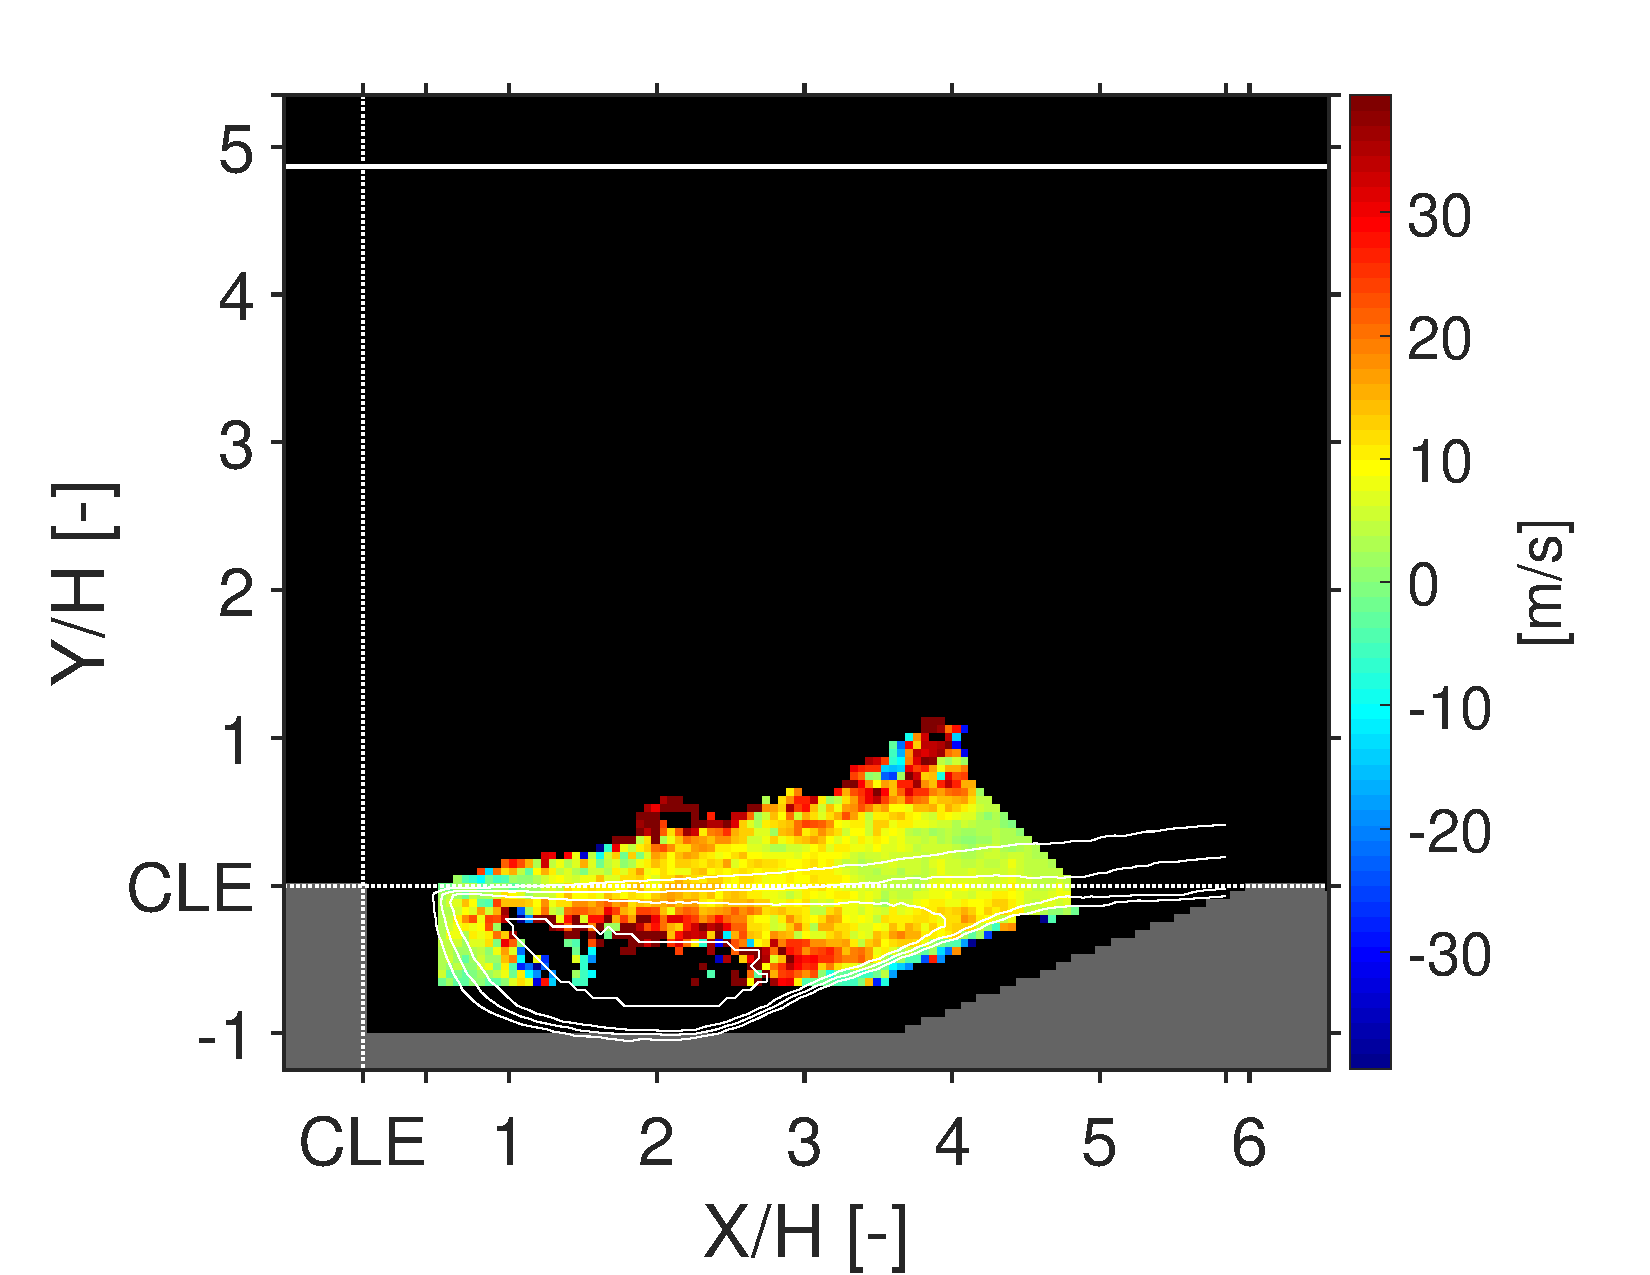
\includegraphics[width=3in,trim=0.35in 0 0.42in 0, clip]{figures/B1/cond_statistics/B1_relative_Uy_AVG_conditional}}
\caption{Mean conditional velocity fields with flame intermittency contours}\label{fig:B2_all_cond_AVG}
\end{figure}

\begin{figure}
\centering
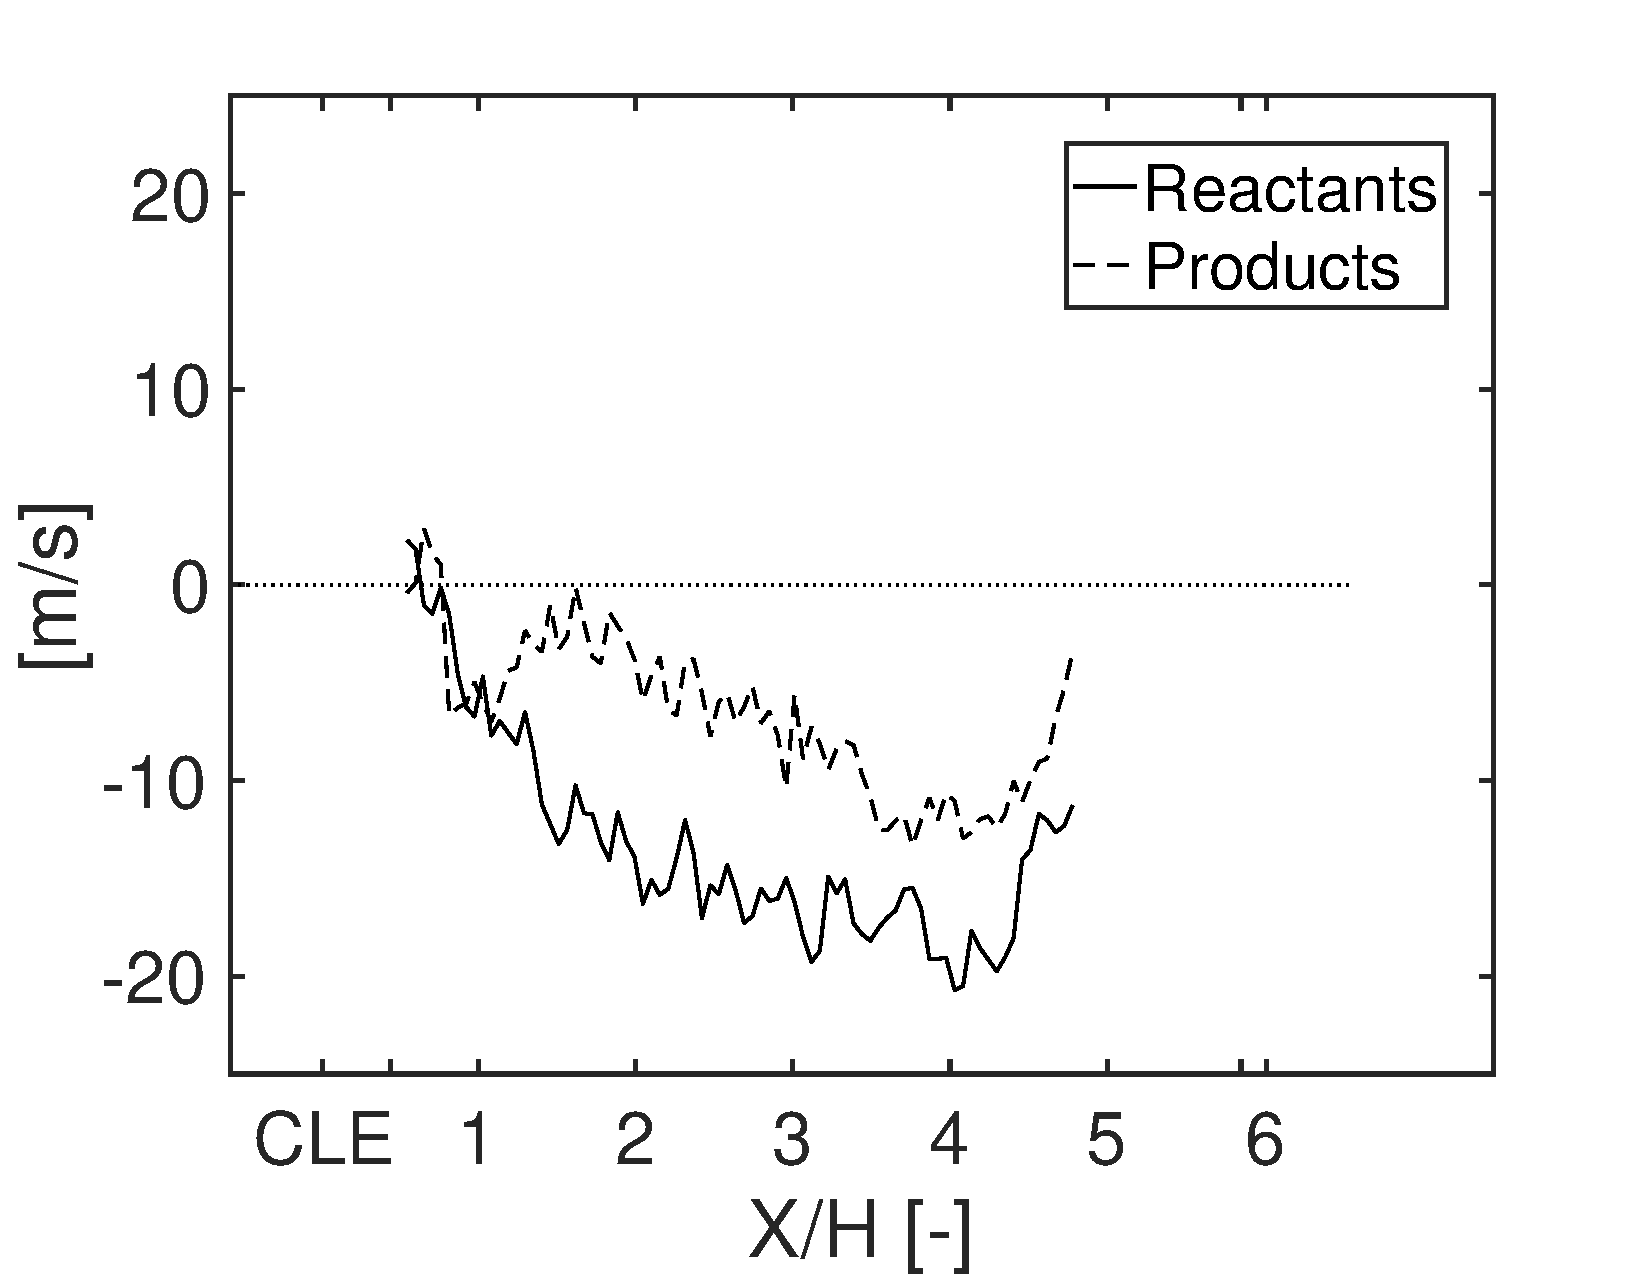
\includegraphics[width=3.25in]{figures/B1/flux/B1_average_YH0_flux} 
\caption{Mean transverse velocities at the cavity interface at $y/H=0$ \label{fig:ch3_cavity_interface_flux}}
\end{figure}
